\section{Can I Rely On You}\label{results:can-i-rely}

\subsection{Infidelity}\label{results:infidelity}

Infidelity (see Section \ref{section:infidelity}) was the first measure used in the experiments. This measure is producing results that are highly sensitive to the data domain and have similar values within the same dataset and model (see Figure \ref{fig:resnet-inf}). This forces us to compare values only within the same dataset and model architecture. Additionally, the comparison of values for the Deconvolution method is  impossible, as shown in the same figure. The reason for that is the way how Deconvolution is calculating the value of attribution. Deconvolution is not using a softmax layer in the calculation, and therefore the absolute output attribution might be a couple of orders of magnitude higher than other methods. In the rest of the section, I am going to remove Deconvolution from the comparison.

\begin{figure}[h]
  \centering
    \centering
    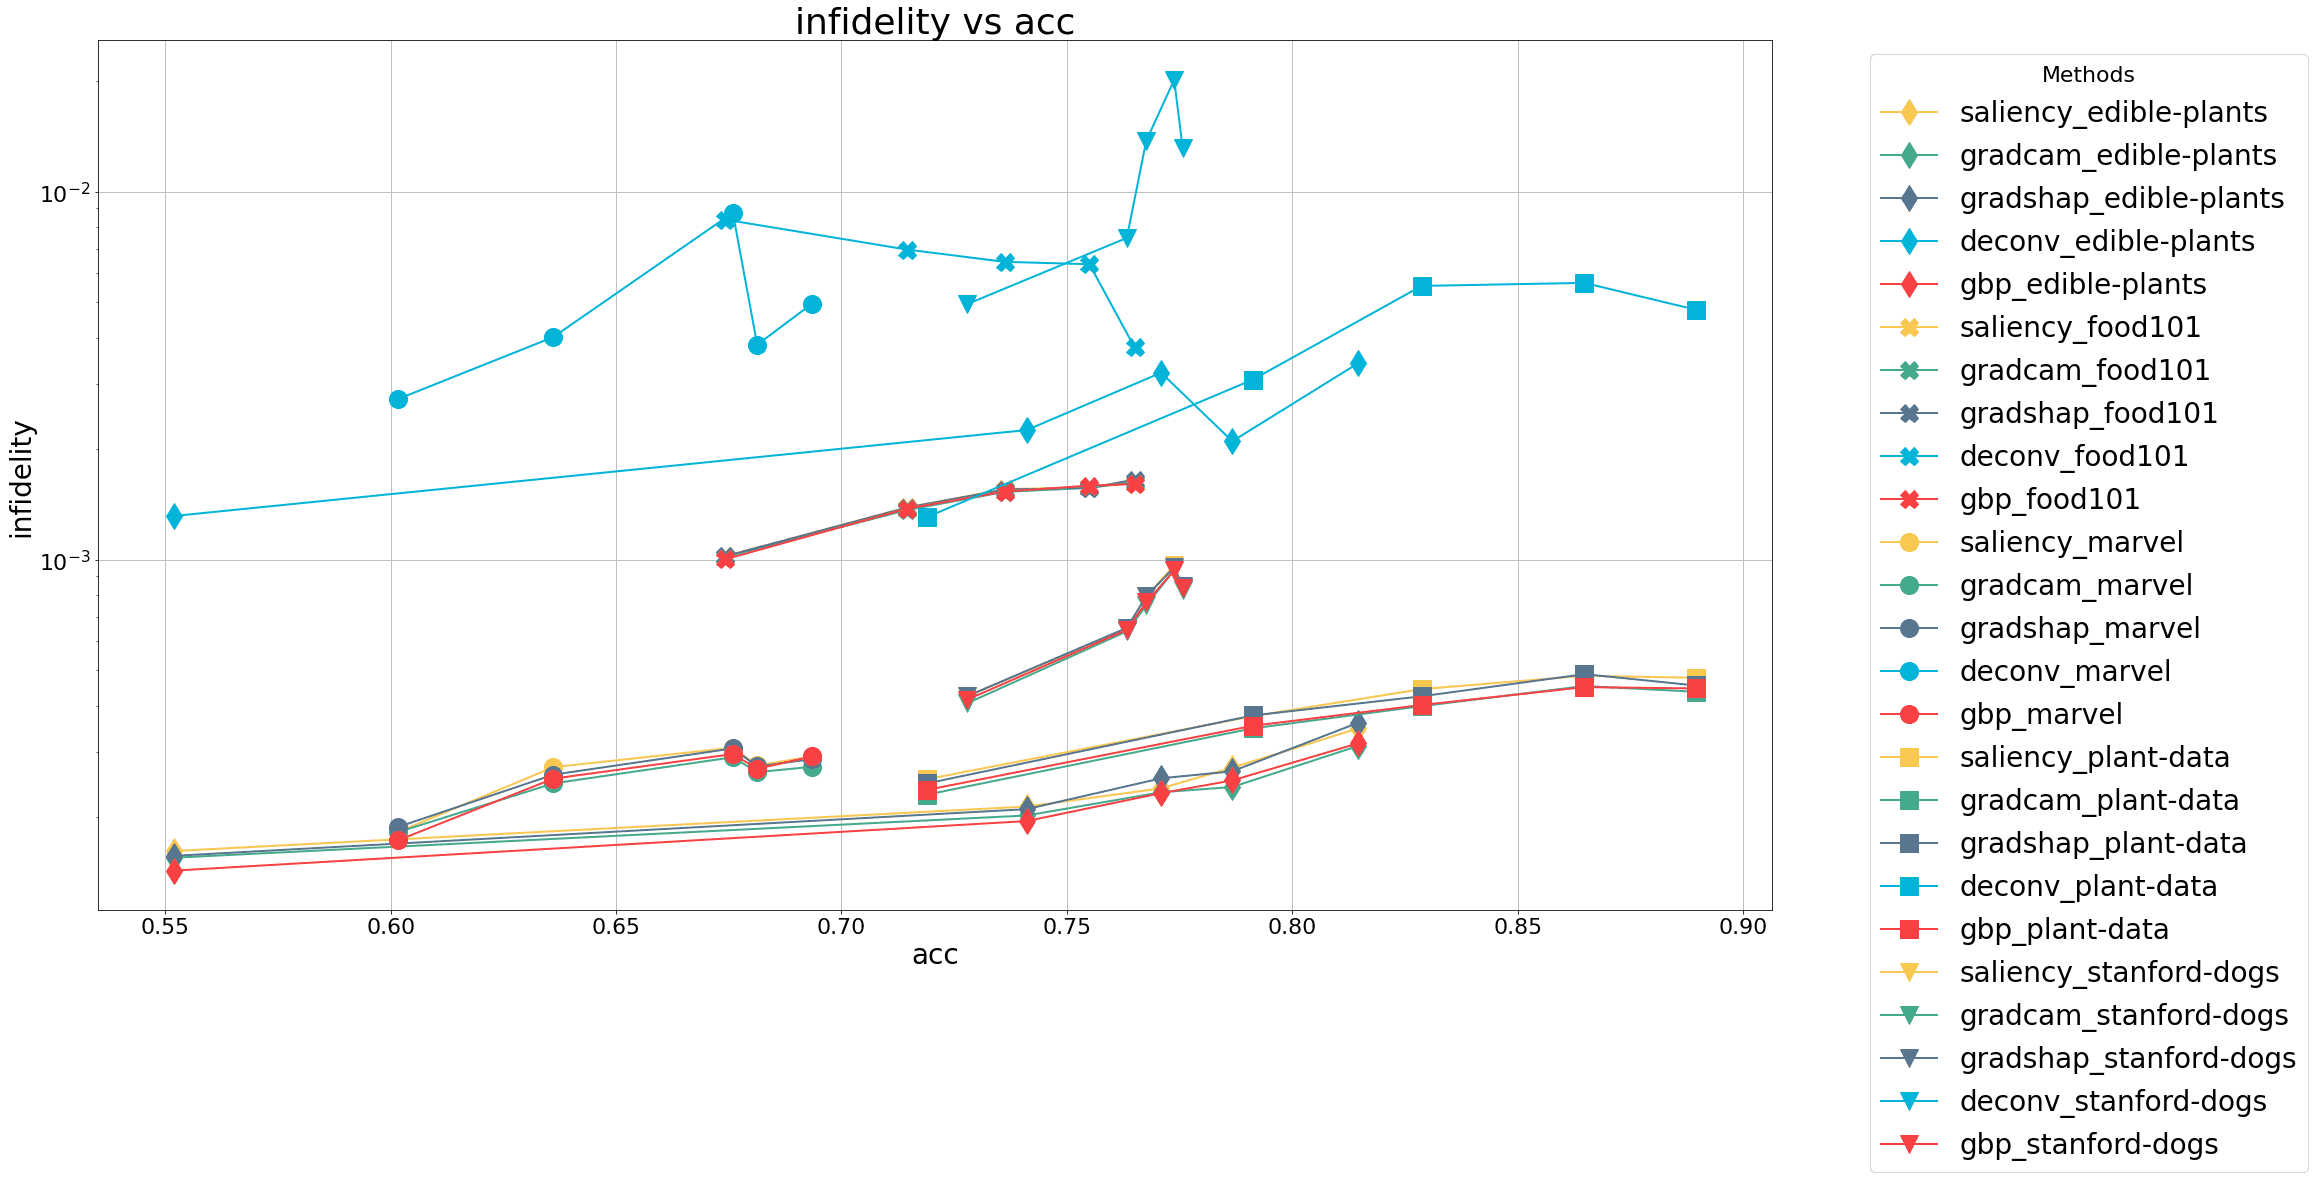
\includegraphics[width=\textwidth]{results/metrics/resnet18-infidelity vs acc.png}
    \caption{Infidelity scores on \textit{ResNet18} architecture. All scores are the mean value for the particular model and are related to that models' accuracy (x-axis). Most of the scores for a dataset are within the same range, except for the Deconvolution method (see Section \ref{section:deconvolution}).}\label{fig:resnet-inf}
\end{figure}

Because comparing the mean infidelity values from the combined chart is visually difficult (see Figure \ref{fig:resnet-inf}), a set of sub-charts was created. All sub-charts can be found in Appendix \ref{fig:combined-infidelity}, because the results on all of them are similar in terms of importance. We can discuss the measure using only a selected few (see Figure \ref{fig:inf-metrics-examples}). 

\vspace{\baselineskip}

To check whether the infidelity meets the definition of reliable measure (see Def. \ref{def:reliability}), we need to compare relative changes of the mean scores for a set of methods within the same dataset. As shown in Figure \ref{fig:resnet-inf-marvel}, the measure is not reliable according to the definition of reliable measure. The values of mean infidelity are not consistent between different model versions, and if we look at the \textit{Guided Backprop} method, they even changing from being the best to being the worst (with an increase in the accuracy). The same result can be seen in Figure \ref{fig:efficientnet-inf-edible-plants}, where methods are changing order base on the models' accuracy (e.g. Saliency is starting as the best method, then at around $0.78$ accuracy is considered to be the worst, and at $0.81$ accuracy is the second-best). This proves the hypothesis that Infidelity is not a reliable measure to compare the XAI methods. 

\begin{figure}[h]
  \centering
 \begin{subfigure}{.49\textwidth}
    \centering
    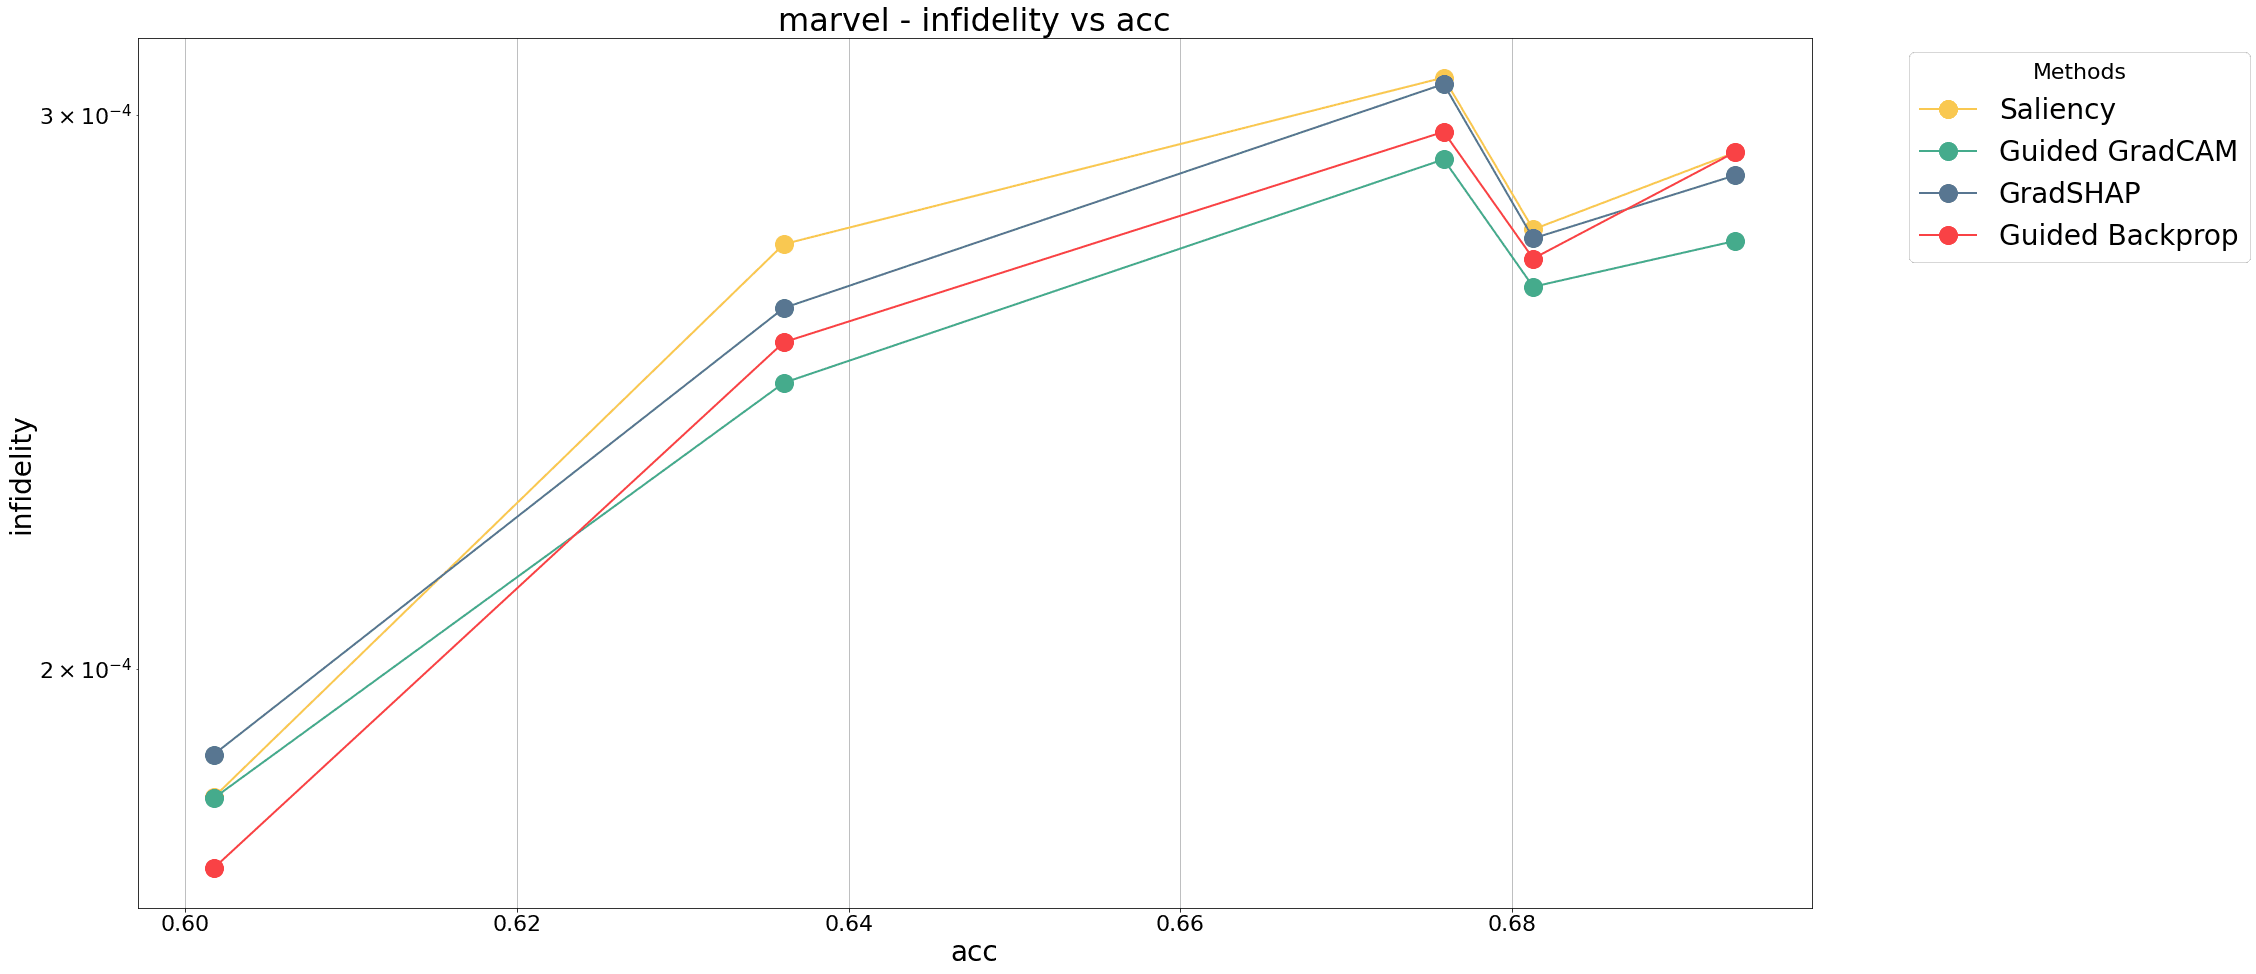
\includegraphics[width=\textwidth]{results/metrics/resnet18-marvel-infidelity vs acc.png}
    \caption{Infidelity scores for \textit{Marvel Heroes} dataset on \textit{ResNet18} architecture}\label{fig:resnet-inf-marvel}
\end{subfigure}
 \begin{subfigure}{.49\textwidth}
    \centering
    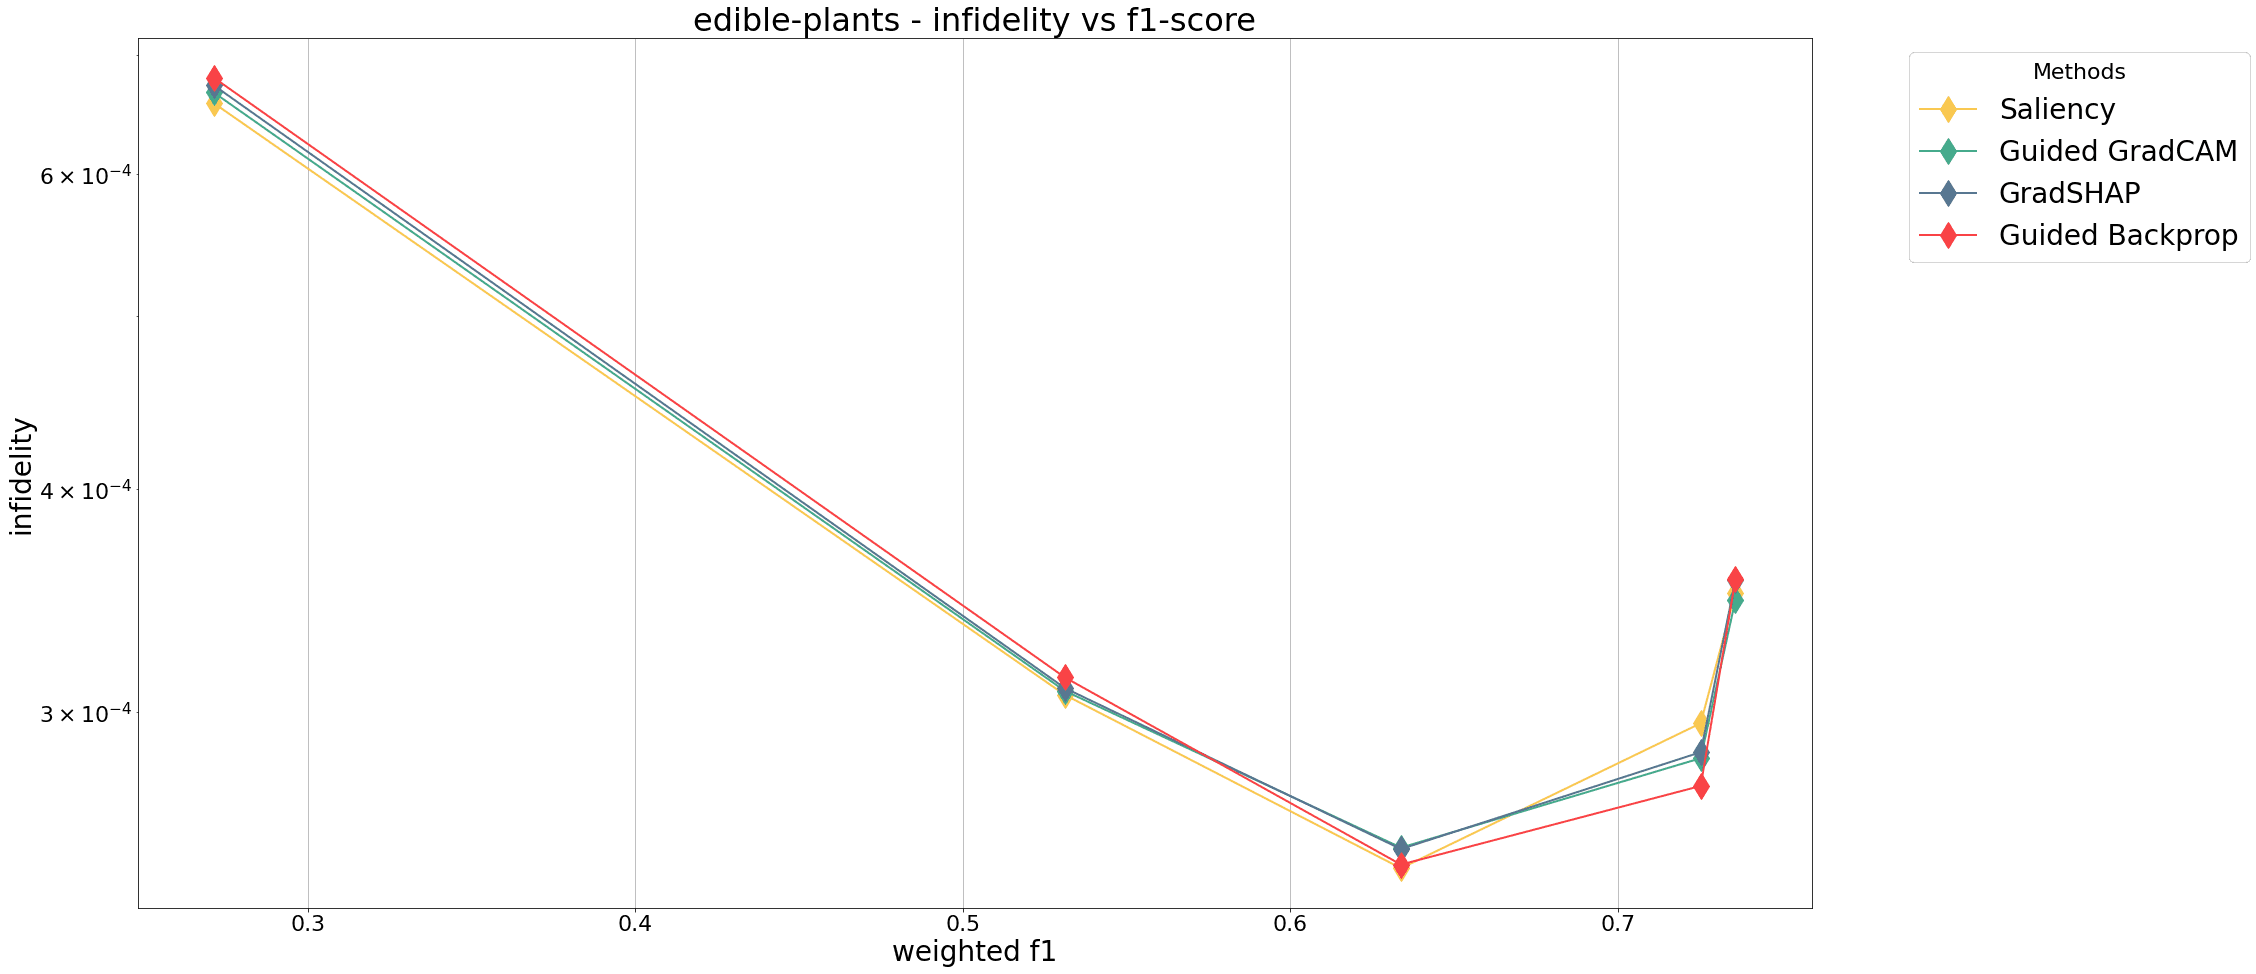
\includegraphics[width=\textwidth]{results/metrics/efficientnet-edible-plants-infidelity vs f1-score.png}
    \caption{Infidelity scores for \textit{Edible wild plants} dataset on \textit{EfficientNet B0} architecture}\label{fig:efficientnet-inf-edible-plants}
\end{subfigure}

 \caption{Sample results for Infidelity measure selected for visualizing the behavior of the measure with the change of model performance. Both charts are showing the relation between the mean infidelity on the test dataset and the models' accuracy on the same dataset.}\label{fig:inf-metrics-examples}
\end{figure}

\vspace{\baselineskip}

Another case against using the infidelity can be seen if we draw the standard deviation of the infidelity measure for all models and methods. As shown in Figure \ref{fig:densenet-inf-std}, a standard deviation is usually similar to the mean value. This makes a single value unreliable when trying to compare it with another value. To visualize this unreliability of values, we can pick particular examples from the dataset. If we look at Figure \ref{fig:resnet-inf-96}, we can see that the value of infidelity for two examples indicated that the explanation provided by the GBP method is better (lower value of infidelity). Both examples are calculated using the same image and the same model version, so there is no discrepancy in models' behavior. Analyzing the attributions, we could agree that the GBP method provides a better explanation (Fig. \ref{fig:resnet-inf-96-gbp}) because it shows more details from the input image than Guided GradCAM (Fig. \ref{fig:resnet-inf-96-gradcam}). This kind of example would be perfect when trying to convince that the measure is working correctly, but we can pick another image from the test dataset and use the same model and methods to compare infidelity values. This time the comparison is between values for the \textit{mallow} class (Fig. \ref{fig:resnet-inf-107}). The infidelity value for GradCAM (Fig. \ref{fig:resnet-inf-107-gradcam}) is much lower than the value for GBP (\ref{fig:resnet-inf-107-gbp}), and once again, GBP shows more details from the input image. In this example, infidelity indicates that an explanation from GBP is much worse than an explanation from GradCAM, and this can be argued when looking at the attributions.

\begin{remark}
Indication of which explanation is better is just my subjective opinion. Comparing two explanations is a qualitative problem and can vary base on the person comparing the explanations. Provided examples are here to indicate the issue with values and not give an answer to which one is better.
\end{remark}


\begin{figure}[h]
  \centering
 \begin{subfigure}{.45\textwidth}
    \centering
    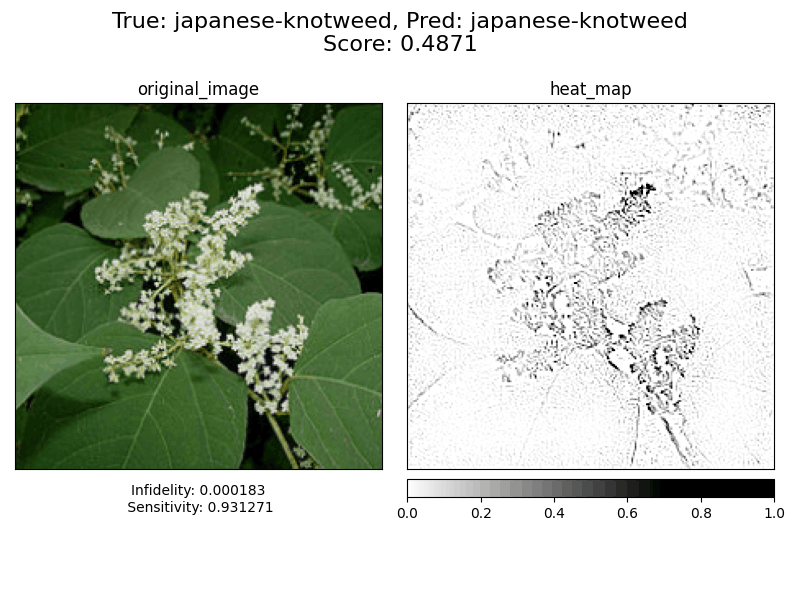
\includegraphics[width=\textwidth]{results/metrics/96-gbp.png}
    \caption{Guided Backprop}\label{fig:resnet-inf-96-gbp}
\end{subfigure}
 \begin{subfigure}{.45\textwidth}
    \centering
    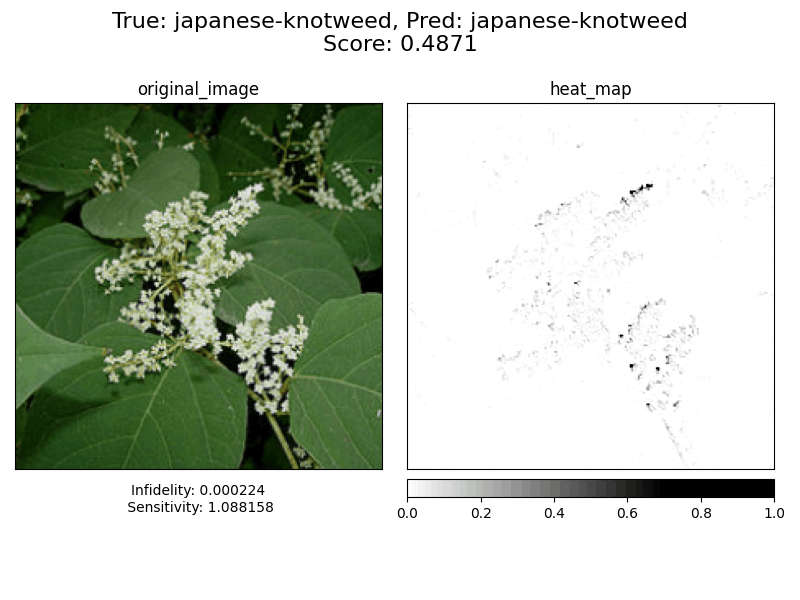
\includegraphics[width=\textwidth]{results/metrics/96-gradcam.png}
    \caption{Guided GradCAM}\label{fig:resnet-inf-96-gradcam}
\end{subfigure}

 \caption{Attributions with assigned infidelity and sensitivity values for a given XAI method. All attributions are generated using \textit{ResNet18} trained with 100\% of training data. Results for the class \textit{japanese-knotweed} from \textit{Edible wild plants} \cite{edible-wild-plants}.}\label{fig:resnet-inf-96}
\end{figure}

\begin{figure}[h]
  \centering
 \begin{subfigure}{.45\textwidth}
    \centering
    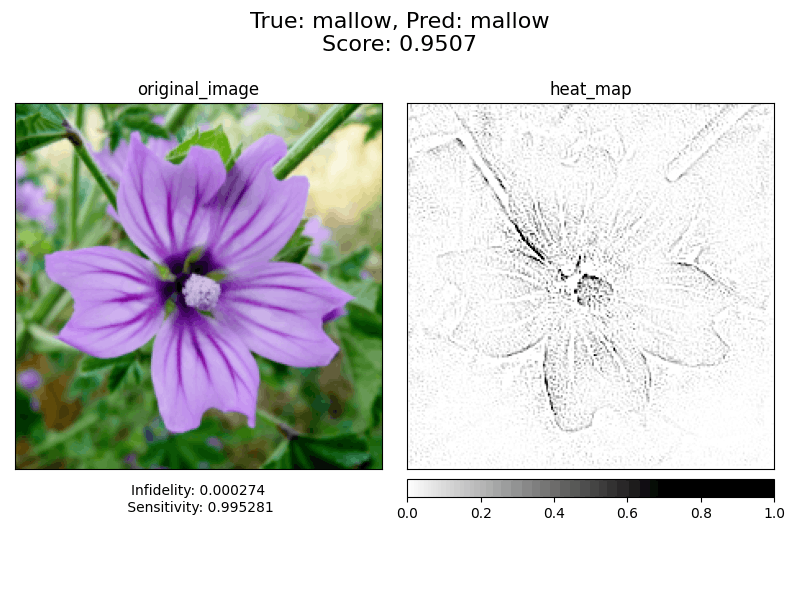
\includegraphics[width=\textwidth]{results/metrics/107-gbp.png}
    \caption{Guided Backprop}\label{fig:resnet-inf-107-gbp}
\end{subfigure}
 \begin{subfigure}{.45\textwidth}
    \centering
    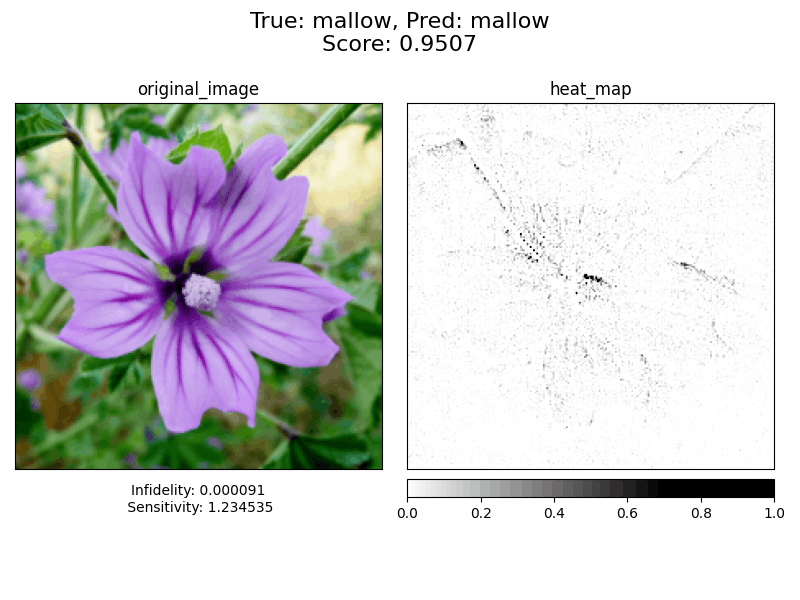
\includegraphics[width=\textwidth]{results/metrics/107-gradcam.png}
    \caption{Guided GradCAM}\label{fig:resnet-inf-107-gradcam}
\end{subfigure}

 \caption{Attributions with assigned infidelity and sensitivity values for a given XAI method. All attributions are generated using \textit{ResNet18} trained with 100\% of training data.  Results for the class \textit{mallow} from \textit{Edible wild plants} \cite{edible-wild-plants}.}\label{fig:resnet-inf-107}
\end{figure}

\begin{figure}[ht]
  \centering
    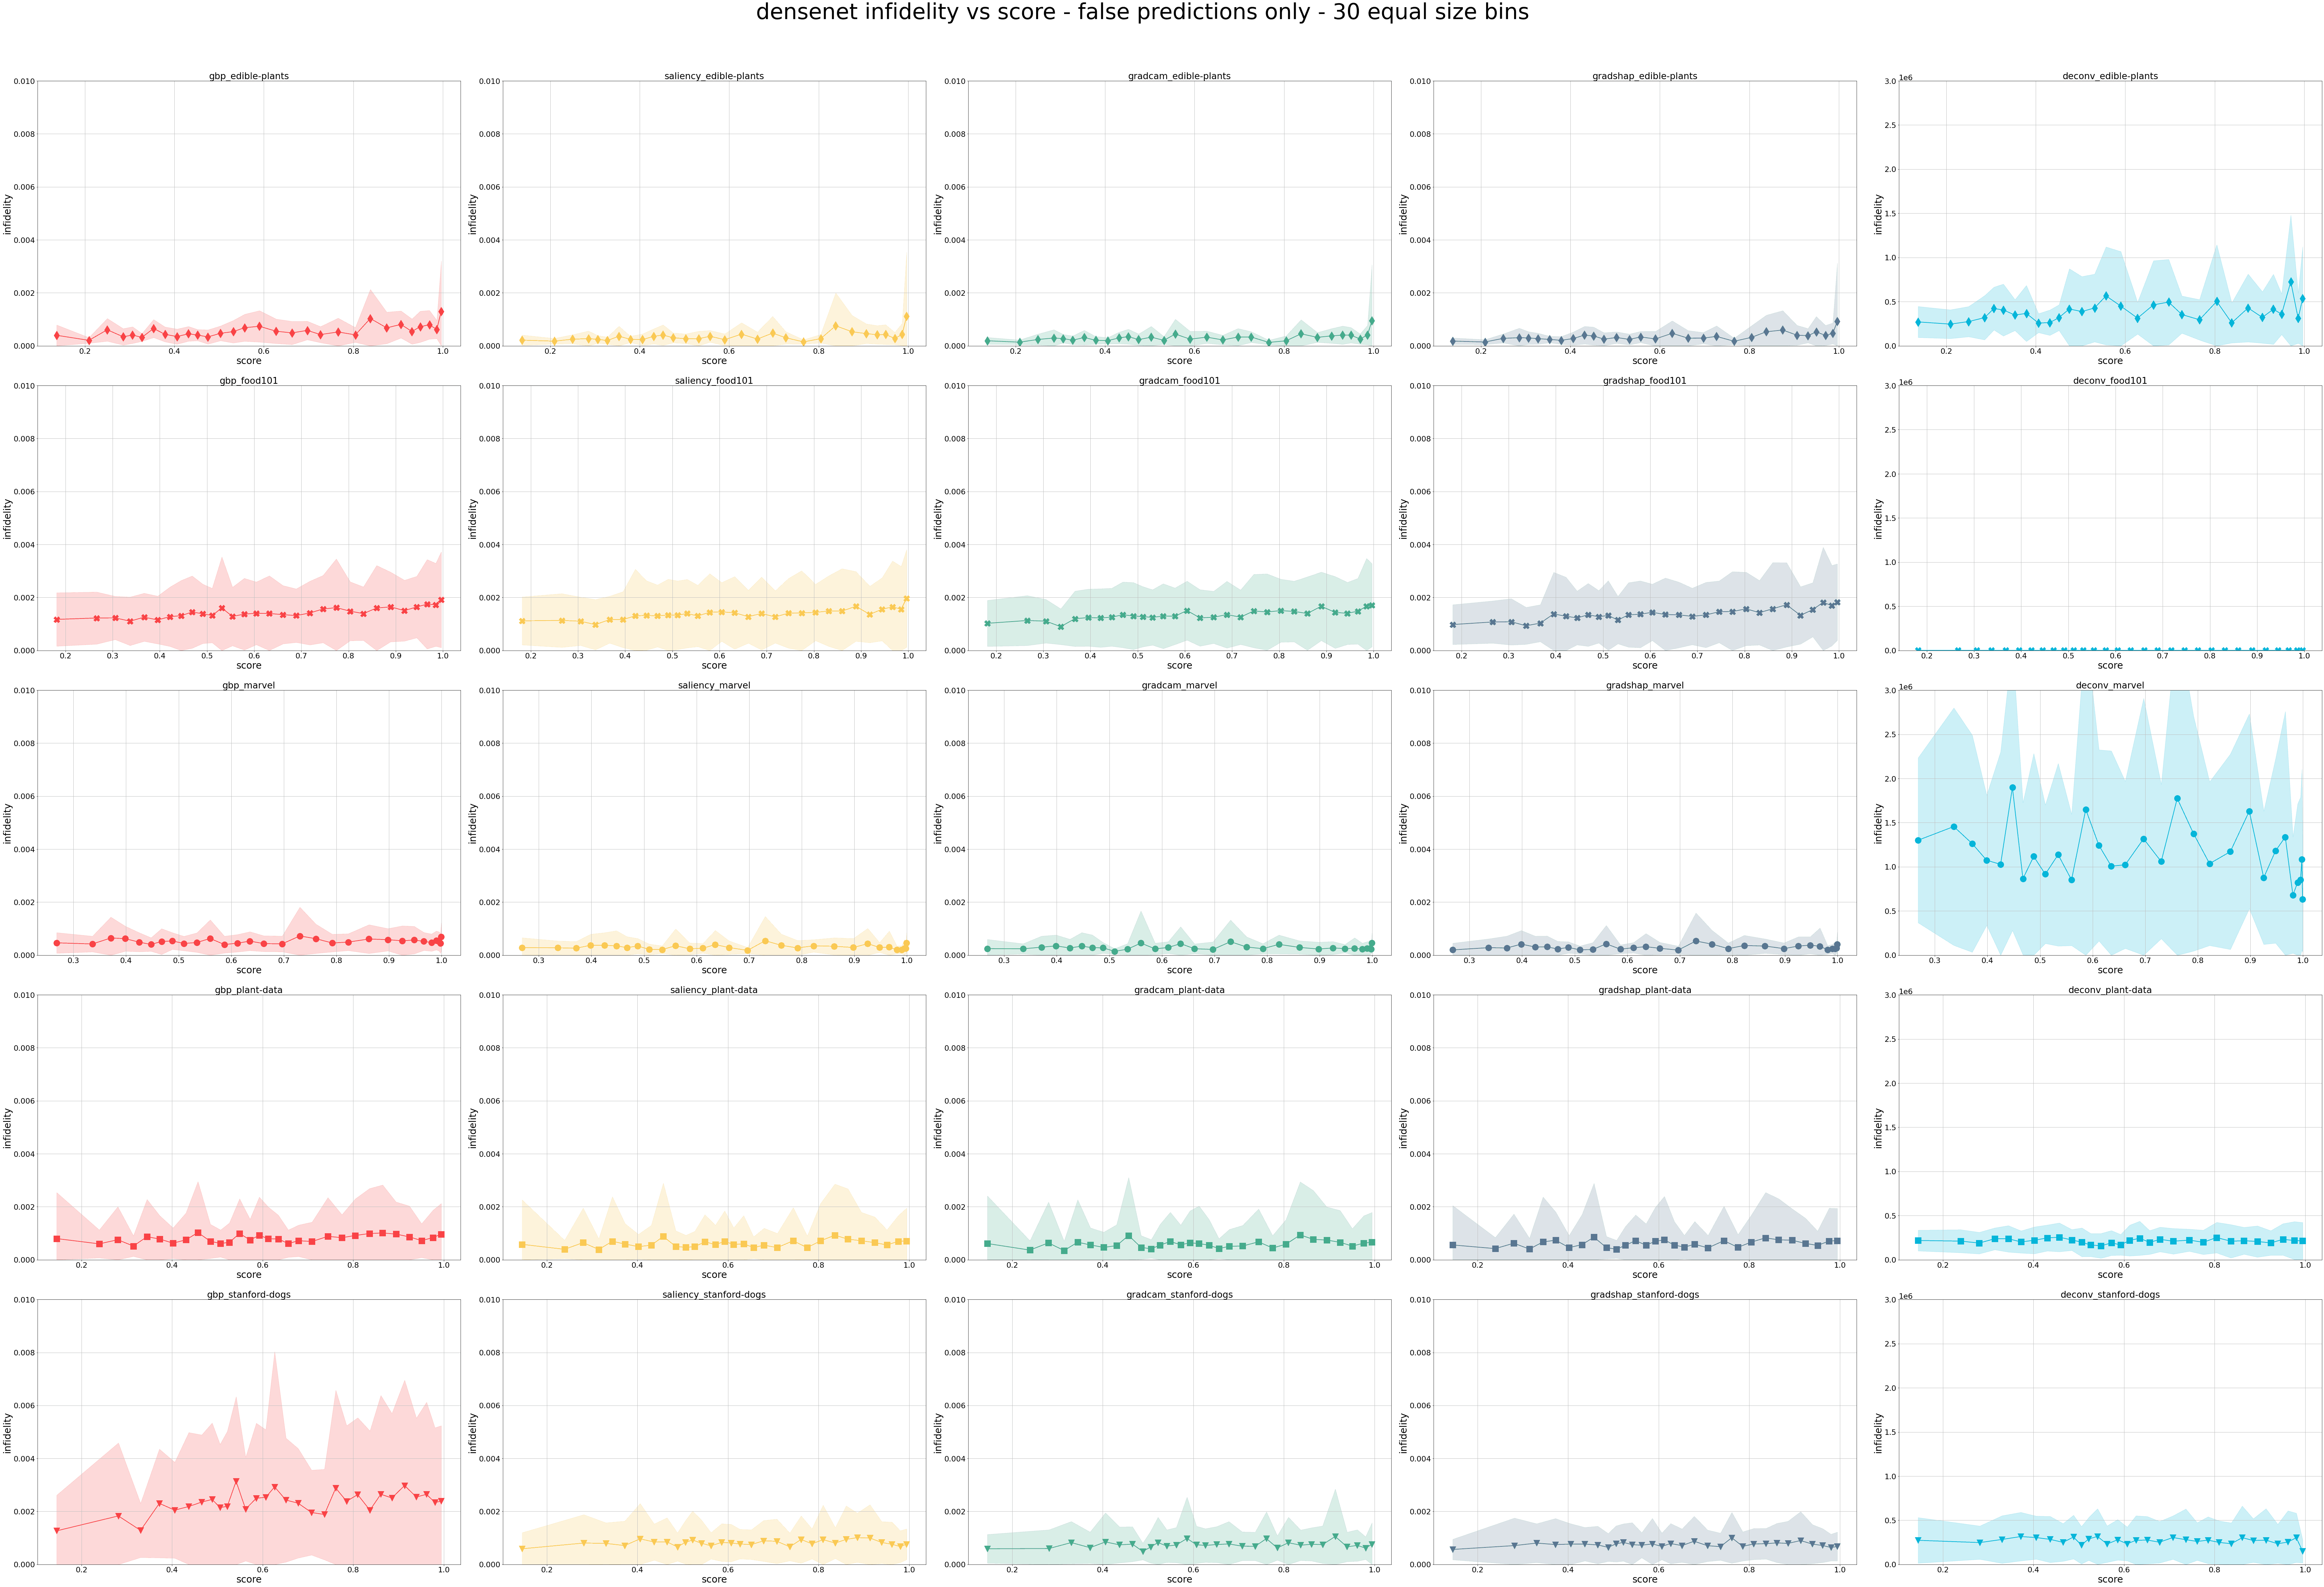
\includegraphics[width=\textwidth]{results/metrics/densenet-infidelity vs score - false predictions only - 30 equal size bins.png}
    \caption{Infidelity scores (with standard deviation) on \textit{DenseNet121} architecture. All scores are the mean value for the particular model and are related to that models' predicted scores (x-axis). Each data point is a mean value of the same amount of samples per dataset. Amounts differ between datasets to always split the results into 30 equally-sized bins.}\label{fig:densenet-inf-std}
\end{figure}


\FloatBarrier

\subsection{Sensitivity}\label{results:sensitivity}

The sensitivity (see Section \ref{section:sensitivity}) measure is more complicated in terms of interpreting the result. Unlike infidelity, which suppose to tell us which XAI method is better, sensitivity measure tells us which XAI method is more prone to change its decision with slight perturbation in the input data. We should keep that in mind when discussing this measure. This time, the Deconvolution method is included in the results because the sensitivity does not have the same issue with an absolute value of attribution as infidelity.

\begin{figure}[ht]
  \centering
    \centering
    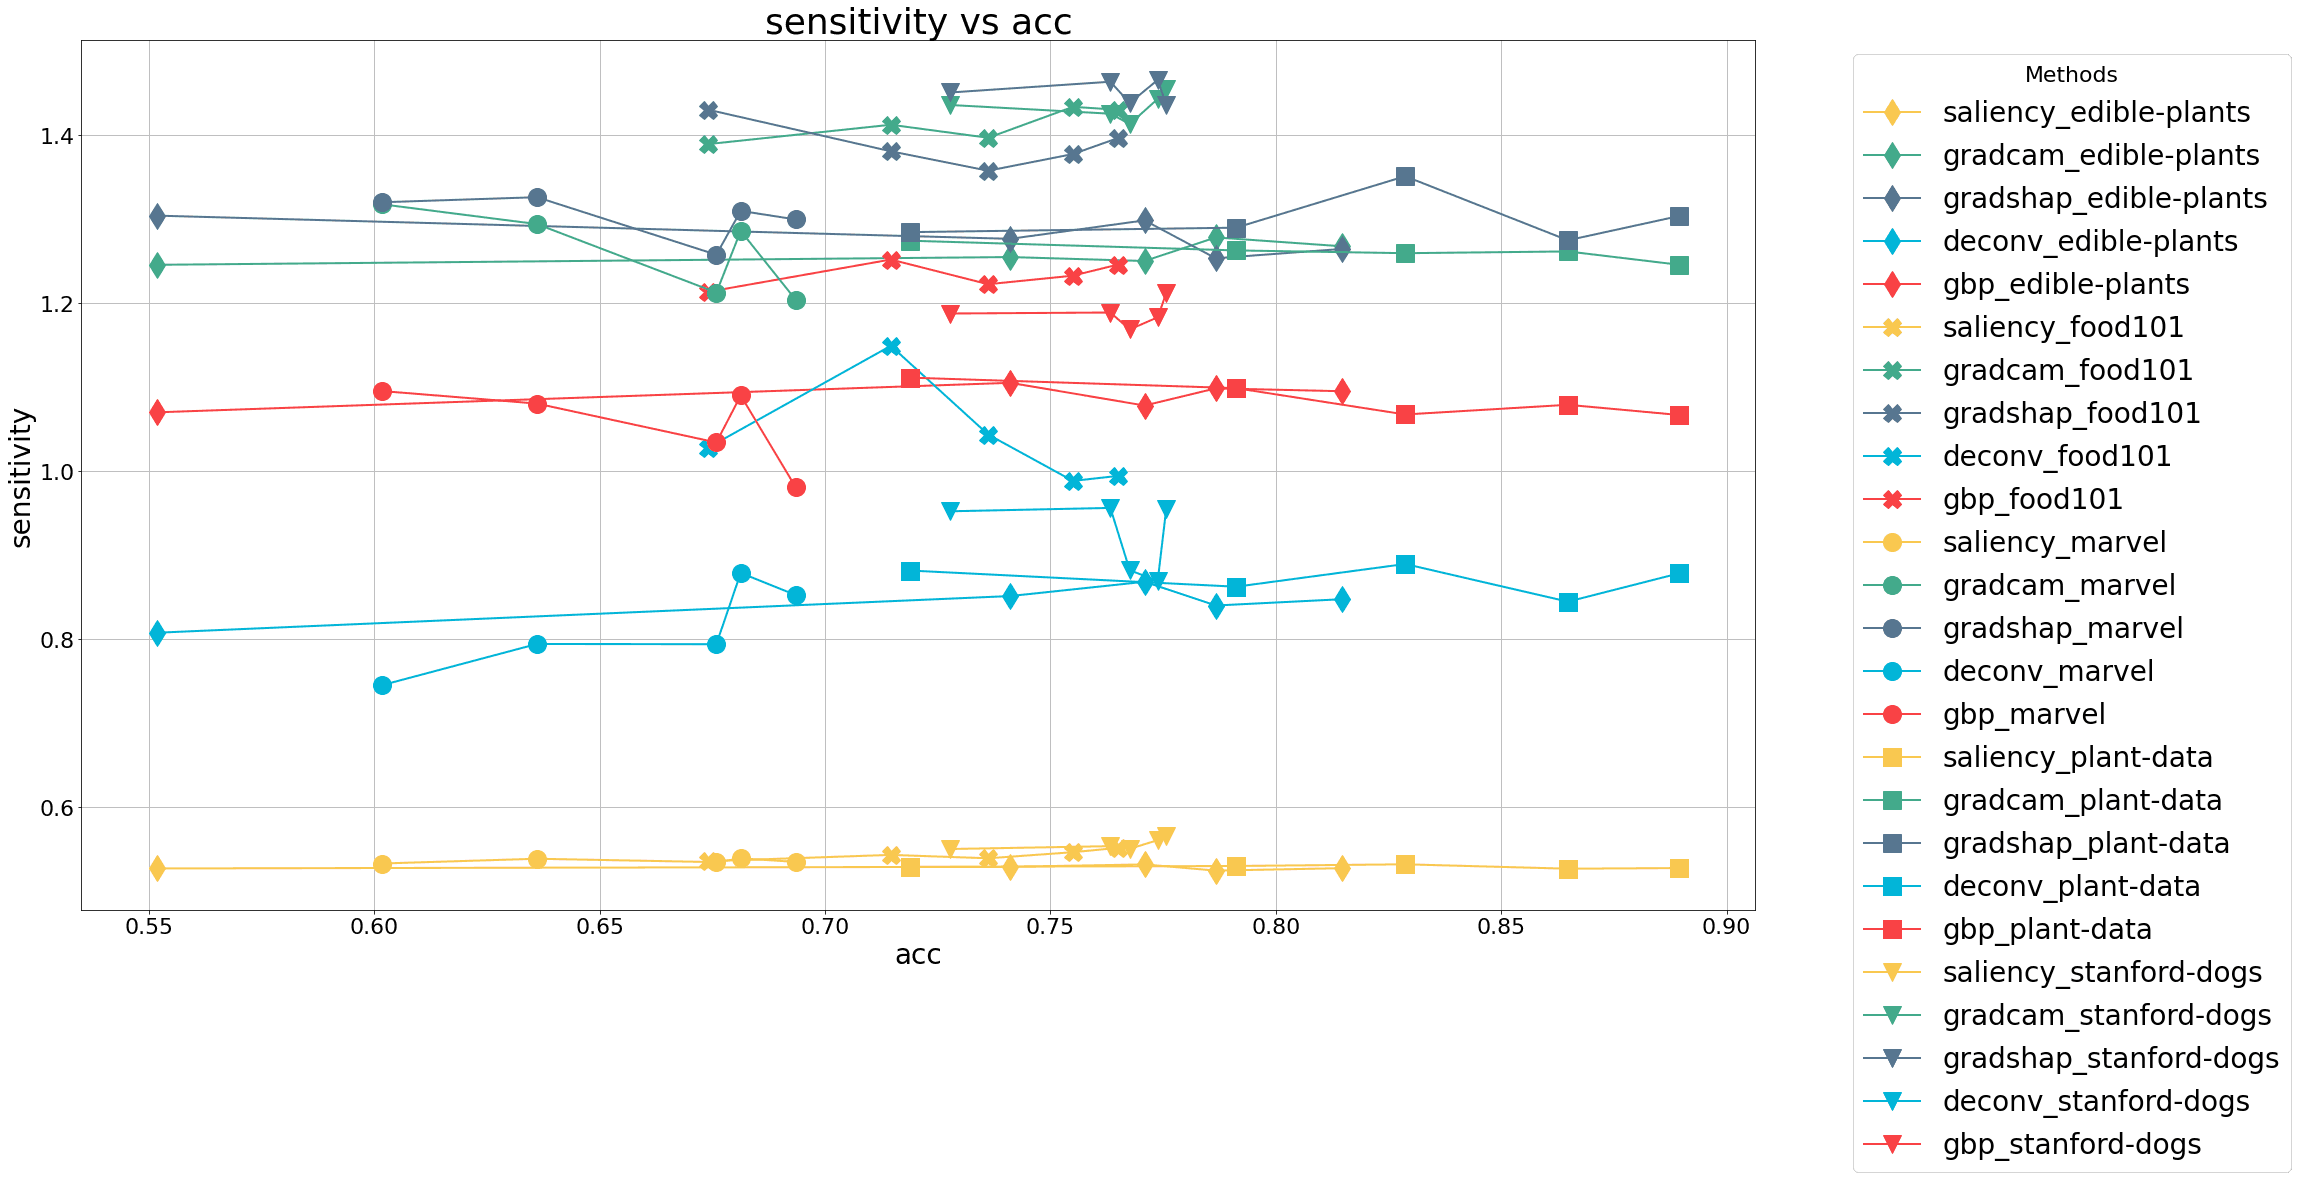
\includegraphics[width=\textwidth]{results/metrics/resnet18-sensitivity vs acc.png}
    \caption{Sensitivity scores on \textit{ResNet18} architecture. All scores are the mean value for the particular model and are related to that models' accuracy (x-axis).}\label{fig:resnet-sens}
\end{figure}

The combined results for the sensitivity shown in Figure \ref{fig:resnet-sens} differ from those for infidelity in Figure \ref{fig:resnet-inf}. This time the data range is not related to the dataset that much, and we can see a distinction between different XAI methods in the form of colored layers. Based on this example, we can decide which XAI method is the most and the less sensitive to input perturbation. It is even easier when we use values that come from the same dataset (see Figure \ref{fig:sens-metrics-examples}). The order of the mean values for XAI methods is preserved between datasets. Even with a small irregularity in Figure \ref{fig:resnet-sens-food101} between GradCAM and GradSHAP values at the low end of the models' accuracy, we can agree that sensitivity is a far better measure in terms of reliability (Def. \ref{def:reliability}) than infidelity.

\vspace{-12pt}
\begin{figure}[ht]
  \centering
 \begin{subfigure}{.40\textwidth}
    \centering
    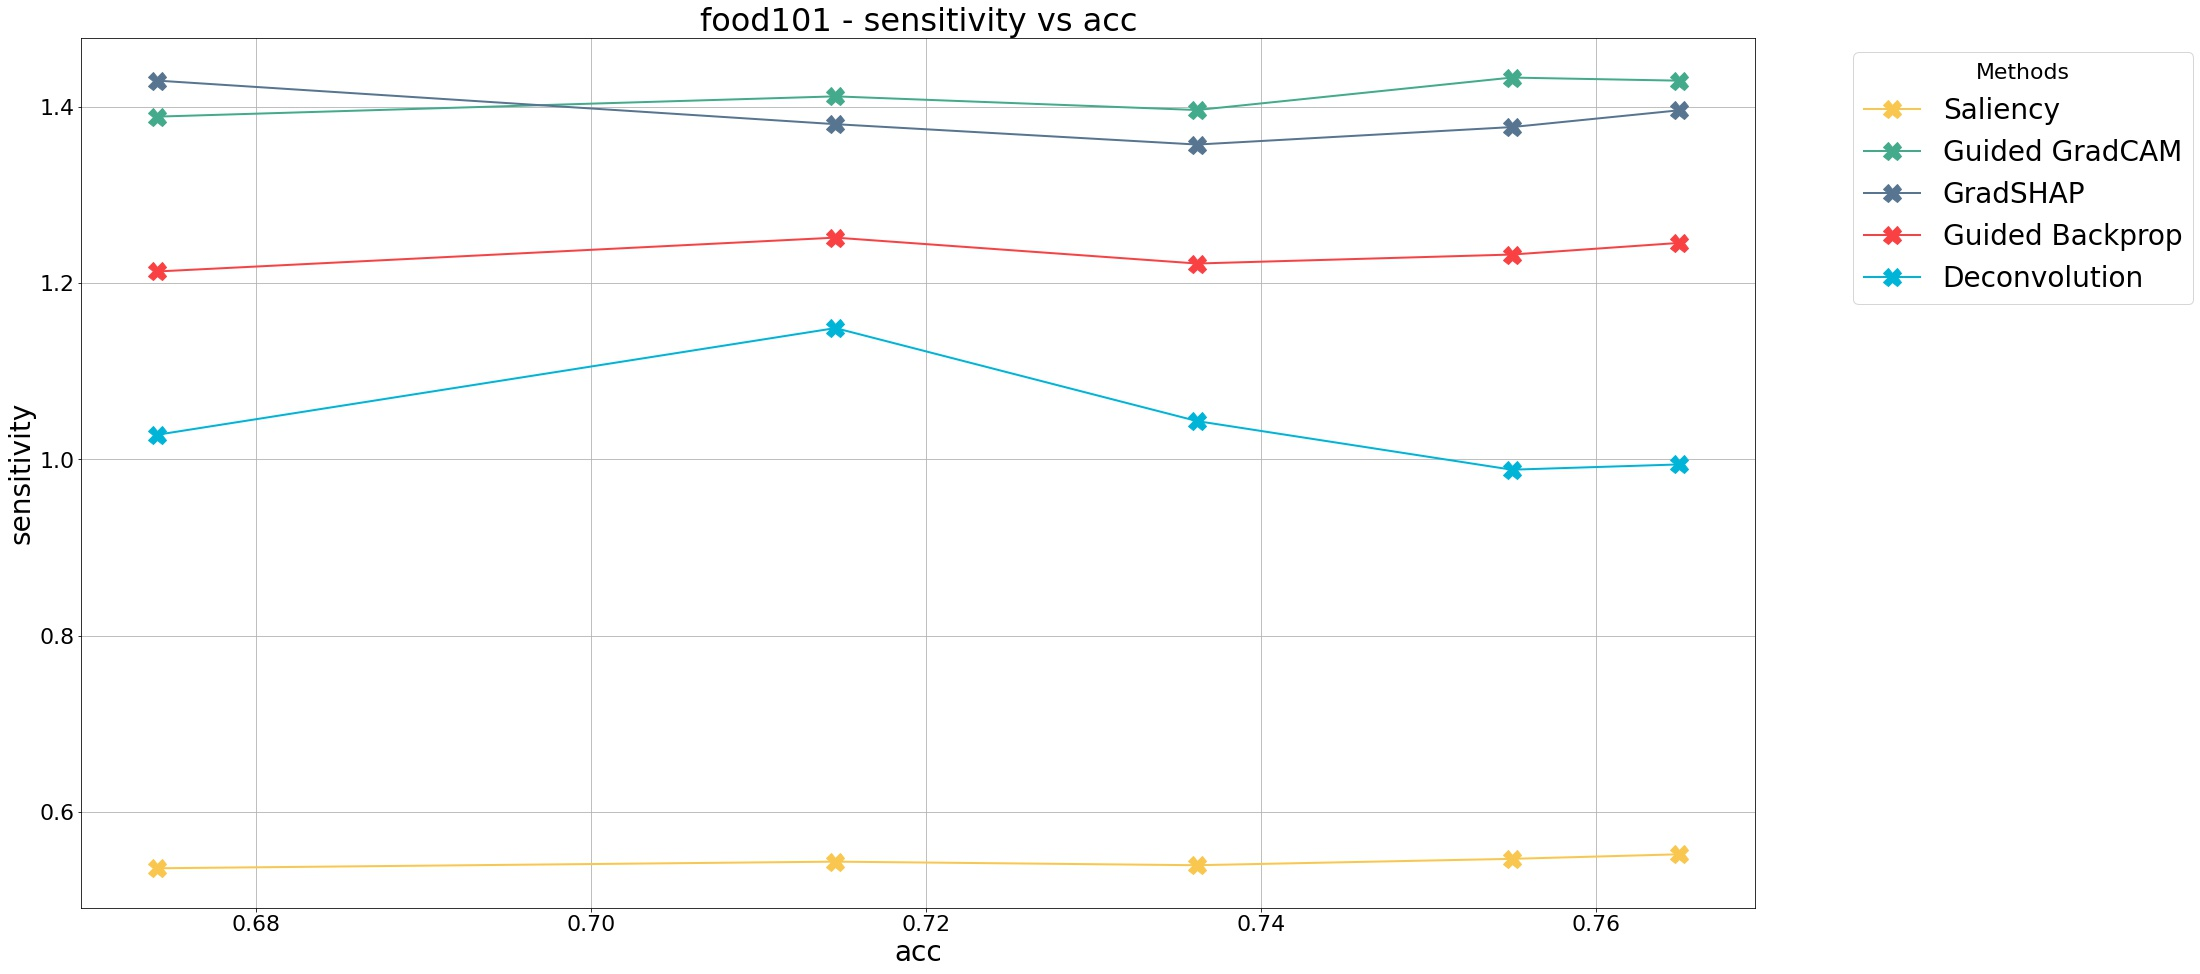
\includegraphics[width=\textwidth]{results/metrics/resnet18-food101-sensitivity vs acc.jpg}
    \caption{Sensitivity scores for \textit{Food101} dataset on \textit{ResNet18} architecture}\label{fig:resnet-sens-food101}
\end{subfigure}
 \begin{subfigure}{.40\textwidth}
    \centering
    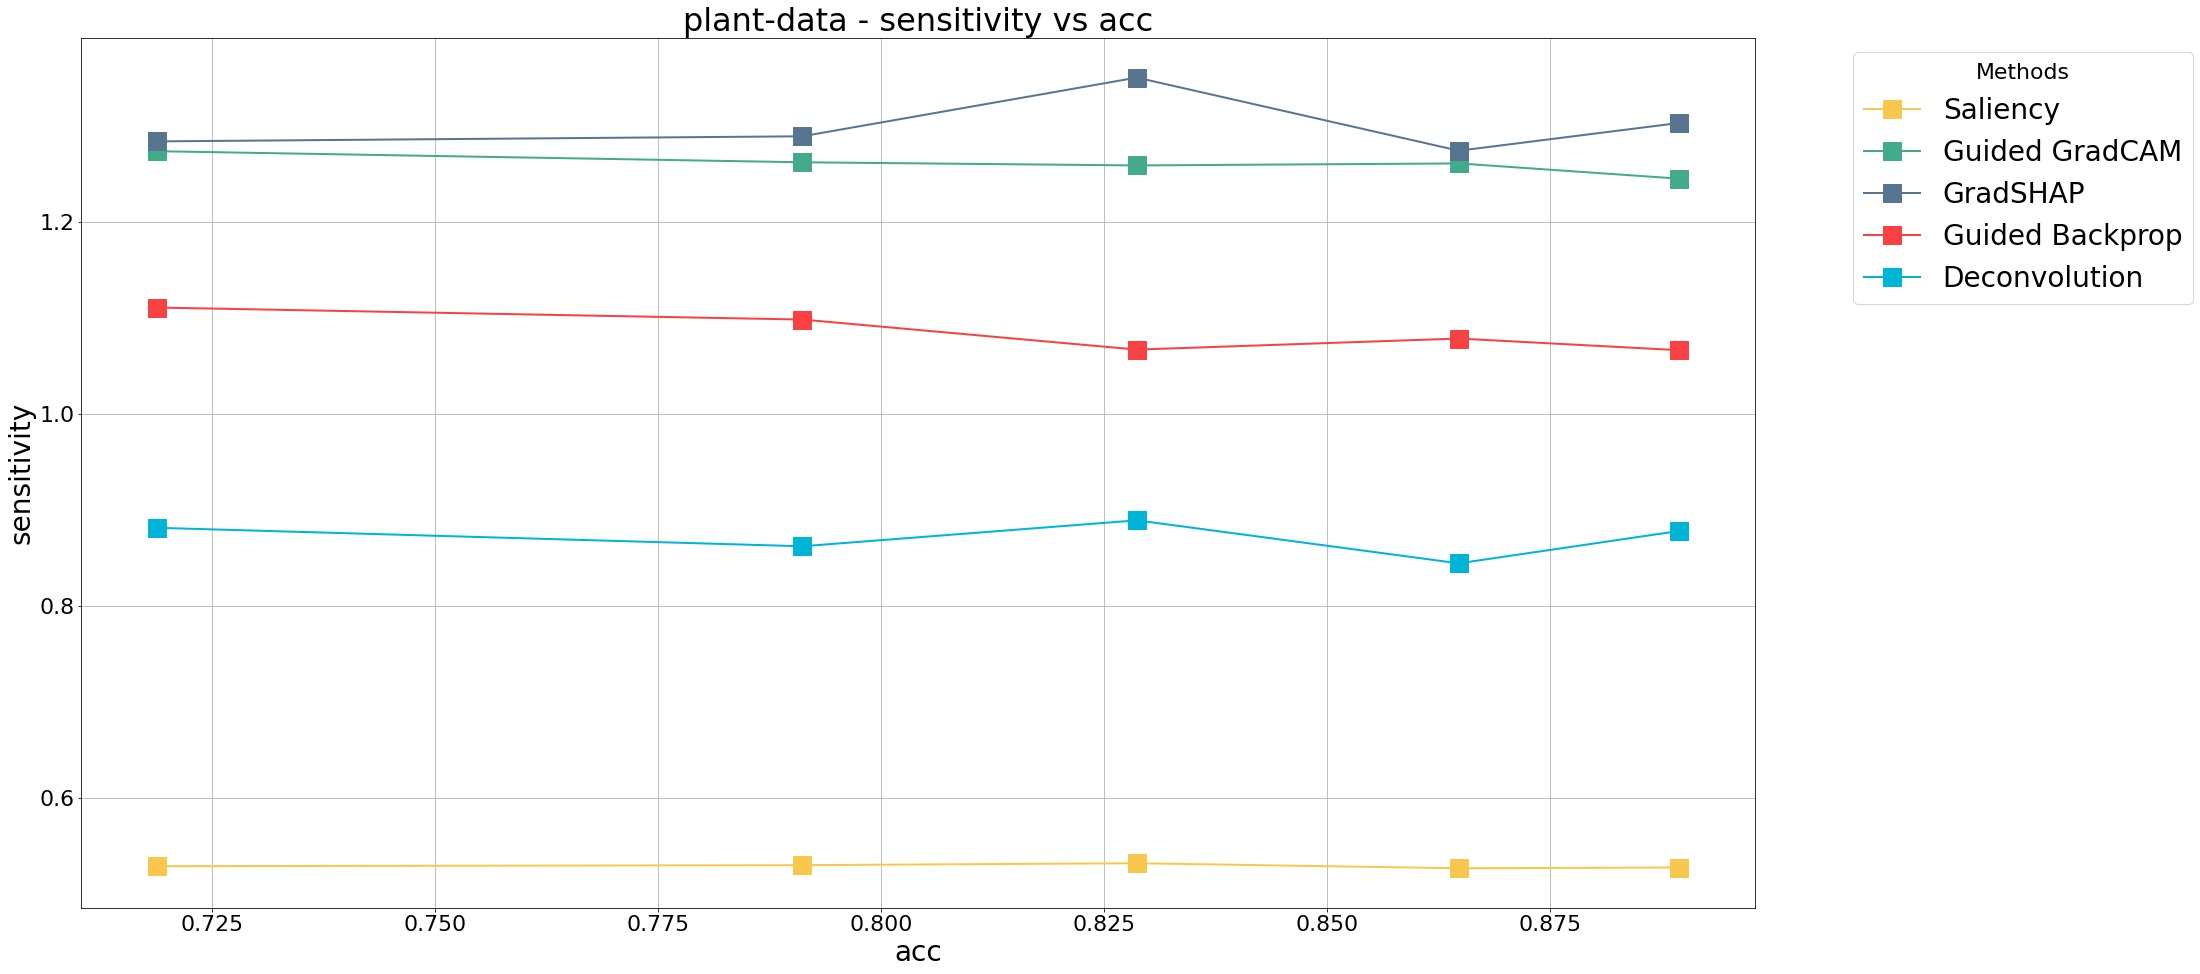
\includegraphics[width=\textwidth]{results/metrics/resnet18-plant-data-sensitivity vs acc.jpg}
    \caption{Sensitivity scores for \textit{Plants} dataset on \textit{ResNet18} architecture}\label{fig:resnet-sens-plants}
\end{subfigure}

 \caption{Sample results for the Sensitivity measure selected for visualizing the behavior of the measure with the change of model performance. Both charts show the relation between the mean sensitivity on the test dataset and the models' accuracy on the same dataset. More individual charts available in Appendix \ref{appendix:combined-sens}.}\label{fig:sens-metrics-examples}
\end{figure}

\FloatBarrier

Unfortunately, this reliability does not apply when trying to compare values between architectures. Figure \ref{fig:efficientnet-sens} shows a different order of XAI methods according to the mean sensitivity value. Saliency is still the least sensitive method, but the rest of the methods did not keep their position. Comparing the orders between two architectures allows us to confirm that hypothesis saying that this measure is not capable of reliable compare XAI methods is true.

\begin{figure}[ht]
  \centering
    \centering
    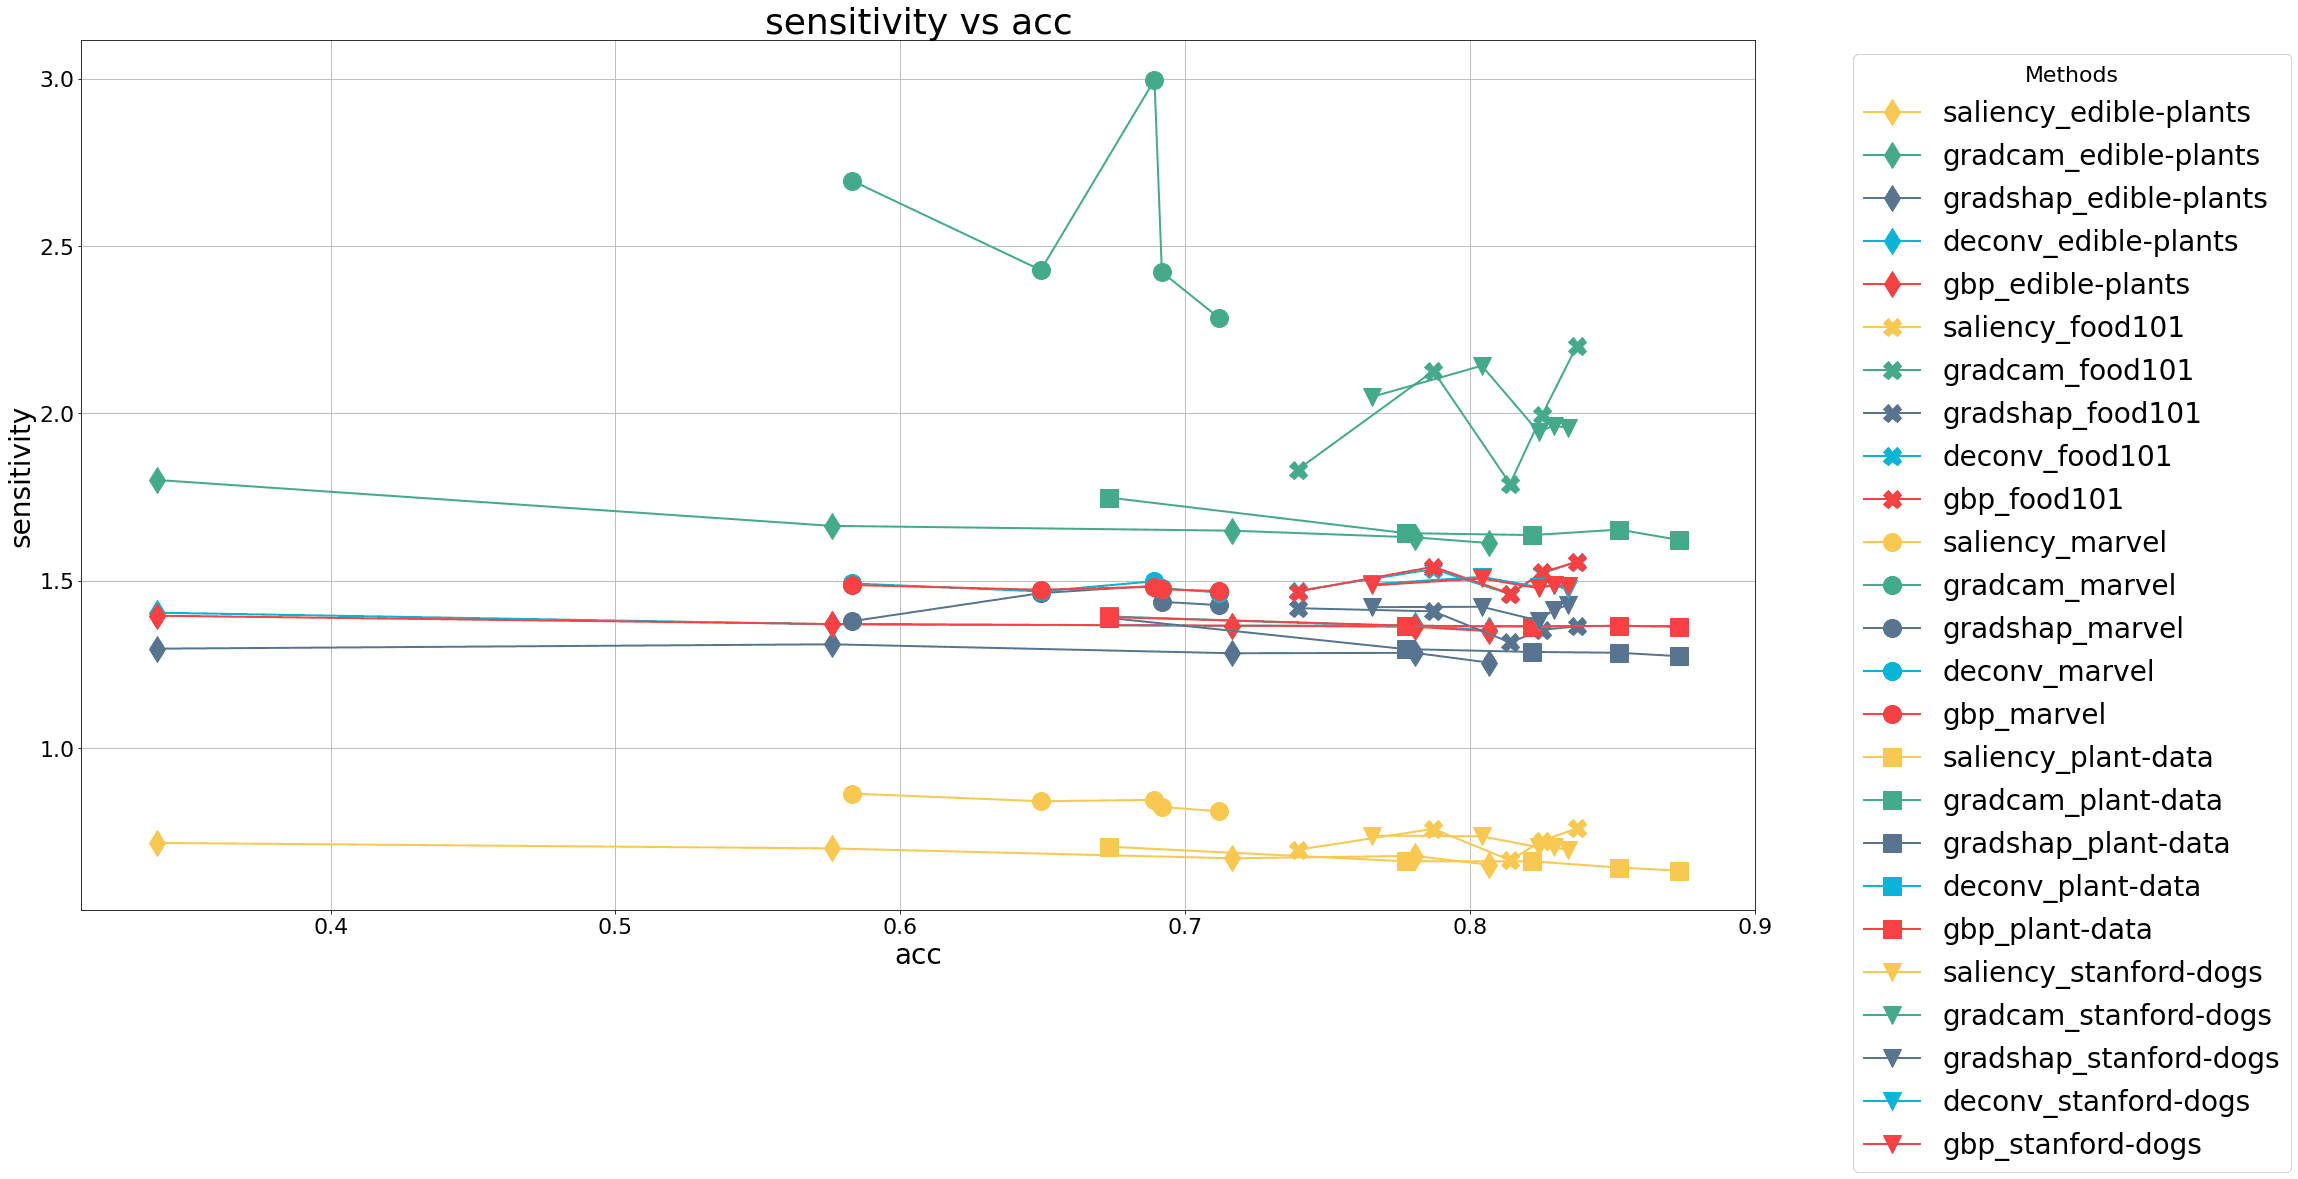
\includegraphics[width=\textwidth]{results/metrics/efficientnet-sensitivity vs acc.png}
    \caption{Sensitivity scores on \textit{EfficientNet B0} architecture. All scores are the mean value for the particular model and are related to that models' accuracy (x-axis).}\label{fig:efficientnet-sens}
\end{figure}

As mentioned at the beginning of this section, sensitivity shows how much a method is sensitive to perturbations in the input data. There is a pattern that can be spotted when looking at the generated examples. Usually, the lower the sensitivity score is, the less accurate the attribution appears to be. As an example, let us compare sensitivity scores for three methods shown in Figure \ref{fig:sens-scores-examples}. An example with the highest sensitivity is a GradCAM (Fig. \ref{fig:sens-score-gradcam}, which has less attribution in total. The method with the lowest sensitivity is always the Saliency (Fig. \ref{fig:sens-score-saliency}) which has more noisy attribution than other methods. This might be caused by the way the sensitivity is calculated. The end value is a total change in attribution after applying perturbation. Methods with fewer attributions (working more like edge detectors) are going to have more attribution change because if the edge is changed, then there is a large difference in value. Methods similar to Saliency, even if the attribution changes, it usually does not change that much because of the initial noise. That might explain differences in mean sensitivity between different models. The attributions produced by the same XAI method usually differ between architectures, and therefore the value of sensitivity is different.

\begin{figure}[ht]
  \centering
 \begin{subfigure}{.3\textwidth}
    \centering
    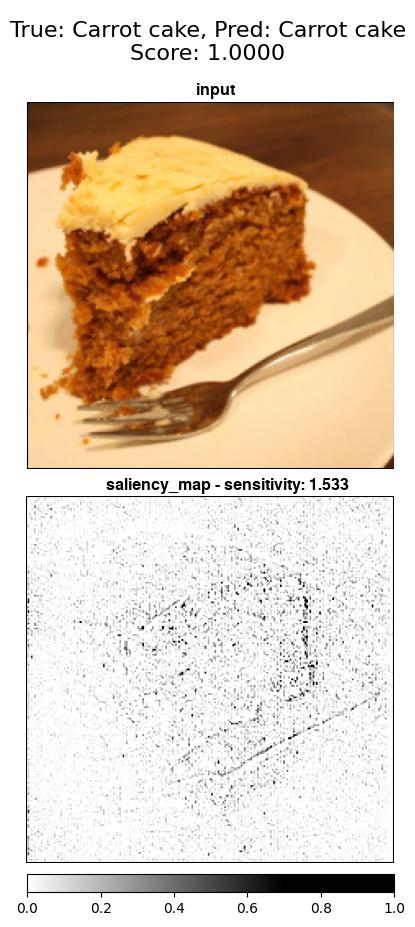
\includegraphics[width=\textwidth]{results/metrics/720-Carrot cake-Carrot cake_vert.jpg}
    \caption{GradCAM}\label{fig:sens-score-gradcam}
\end{subfigure}
 \begin{subfigure}{.31\textwidth}
    \centering
    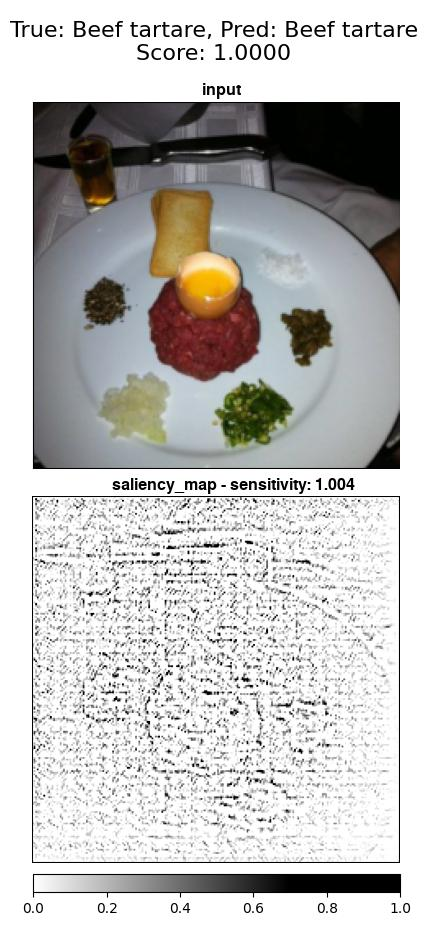
\includegraphics[width=\textwidth]{results/metrics/243-Beef tartare-Beef tartare_vert.jpg}
    \caption{Deconvolution}\label{fig:sens-score-deconv}
\end{subfigure}
 \begin{subfigure}{.345\textwidth}
    \centering
    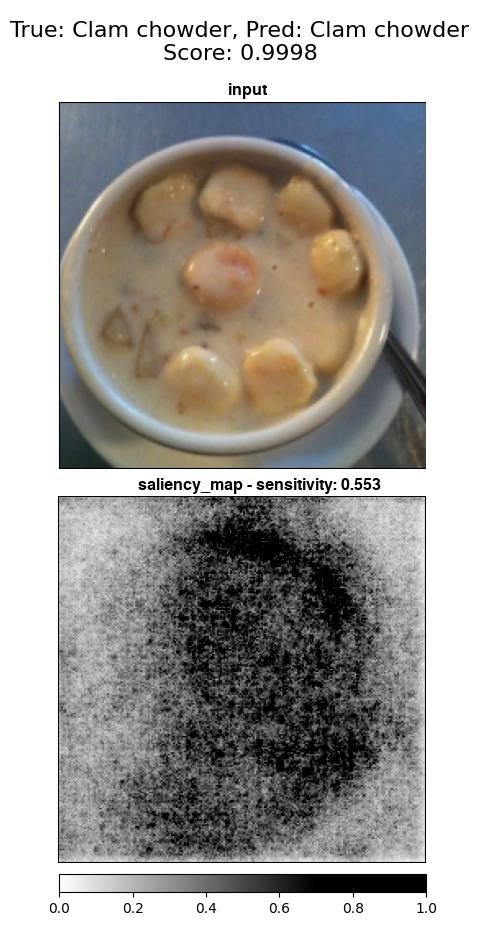
\includegraphics[width=\textwidth]{results/metrics/1246-Clam chowder-Clam chowder_vert.jpg}
    \caption{Saliency}\label{fig:sens-score-saliency}
\end{subfigure}

 \caption{Sensitivity scores for different methods produced for \textit{ResNet18} architecture and examples from \textit{Food101} dataset: \textit{Beef tartare} \ref{fig:sens-score-deconv}, \textit{Carrot cake} \ref{fig:sens-score-gradcam}, \textit{Clam chowder} \ref{fig:sens-score-saliency}.}\label{fig:sens-scores-examples}
\end{figure}

\vspace{\baselineskip}

Additionally, we have to look at the standard deviation of the sensitivity scores (Fig. \ref{fig:resnet-sens-std}). This chart significantly differs from the one showing standard deviation for infidelity. The standard deviation for mean sensitivity measure per score shows that some methods (like Saliency) have low variance in sensitivity when methods with more detailed attributions (like GradCAM) have higher variance. That is related to some methods showing less noise in the attributions. The standard deviation also is dependent on the architecture, and sometimes the values of the deviation might vary a lot. A good example is a chart created for EfficientNet B0 architecture in Figure \ref{fig:efficientnet-sens-std}. Some of the values are outside the value range (GradCAM).

\begin{figure}[ht]
  \centering
    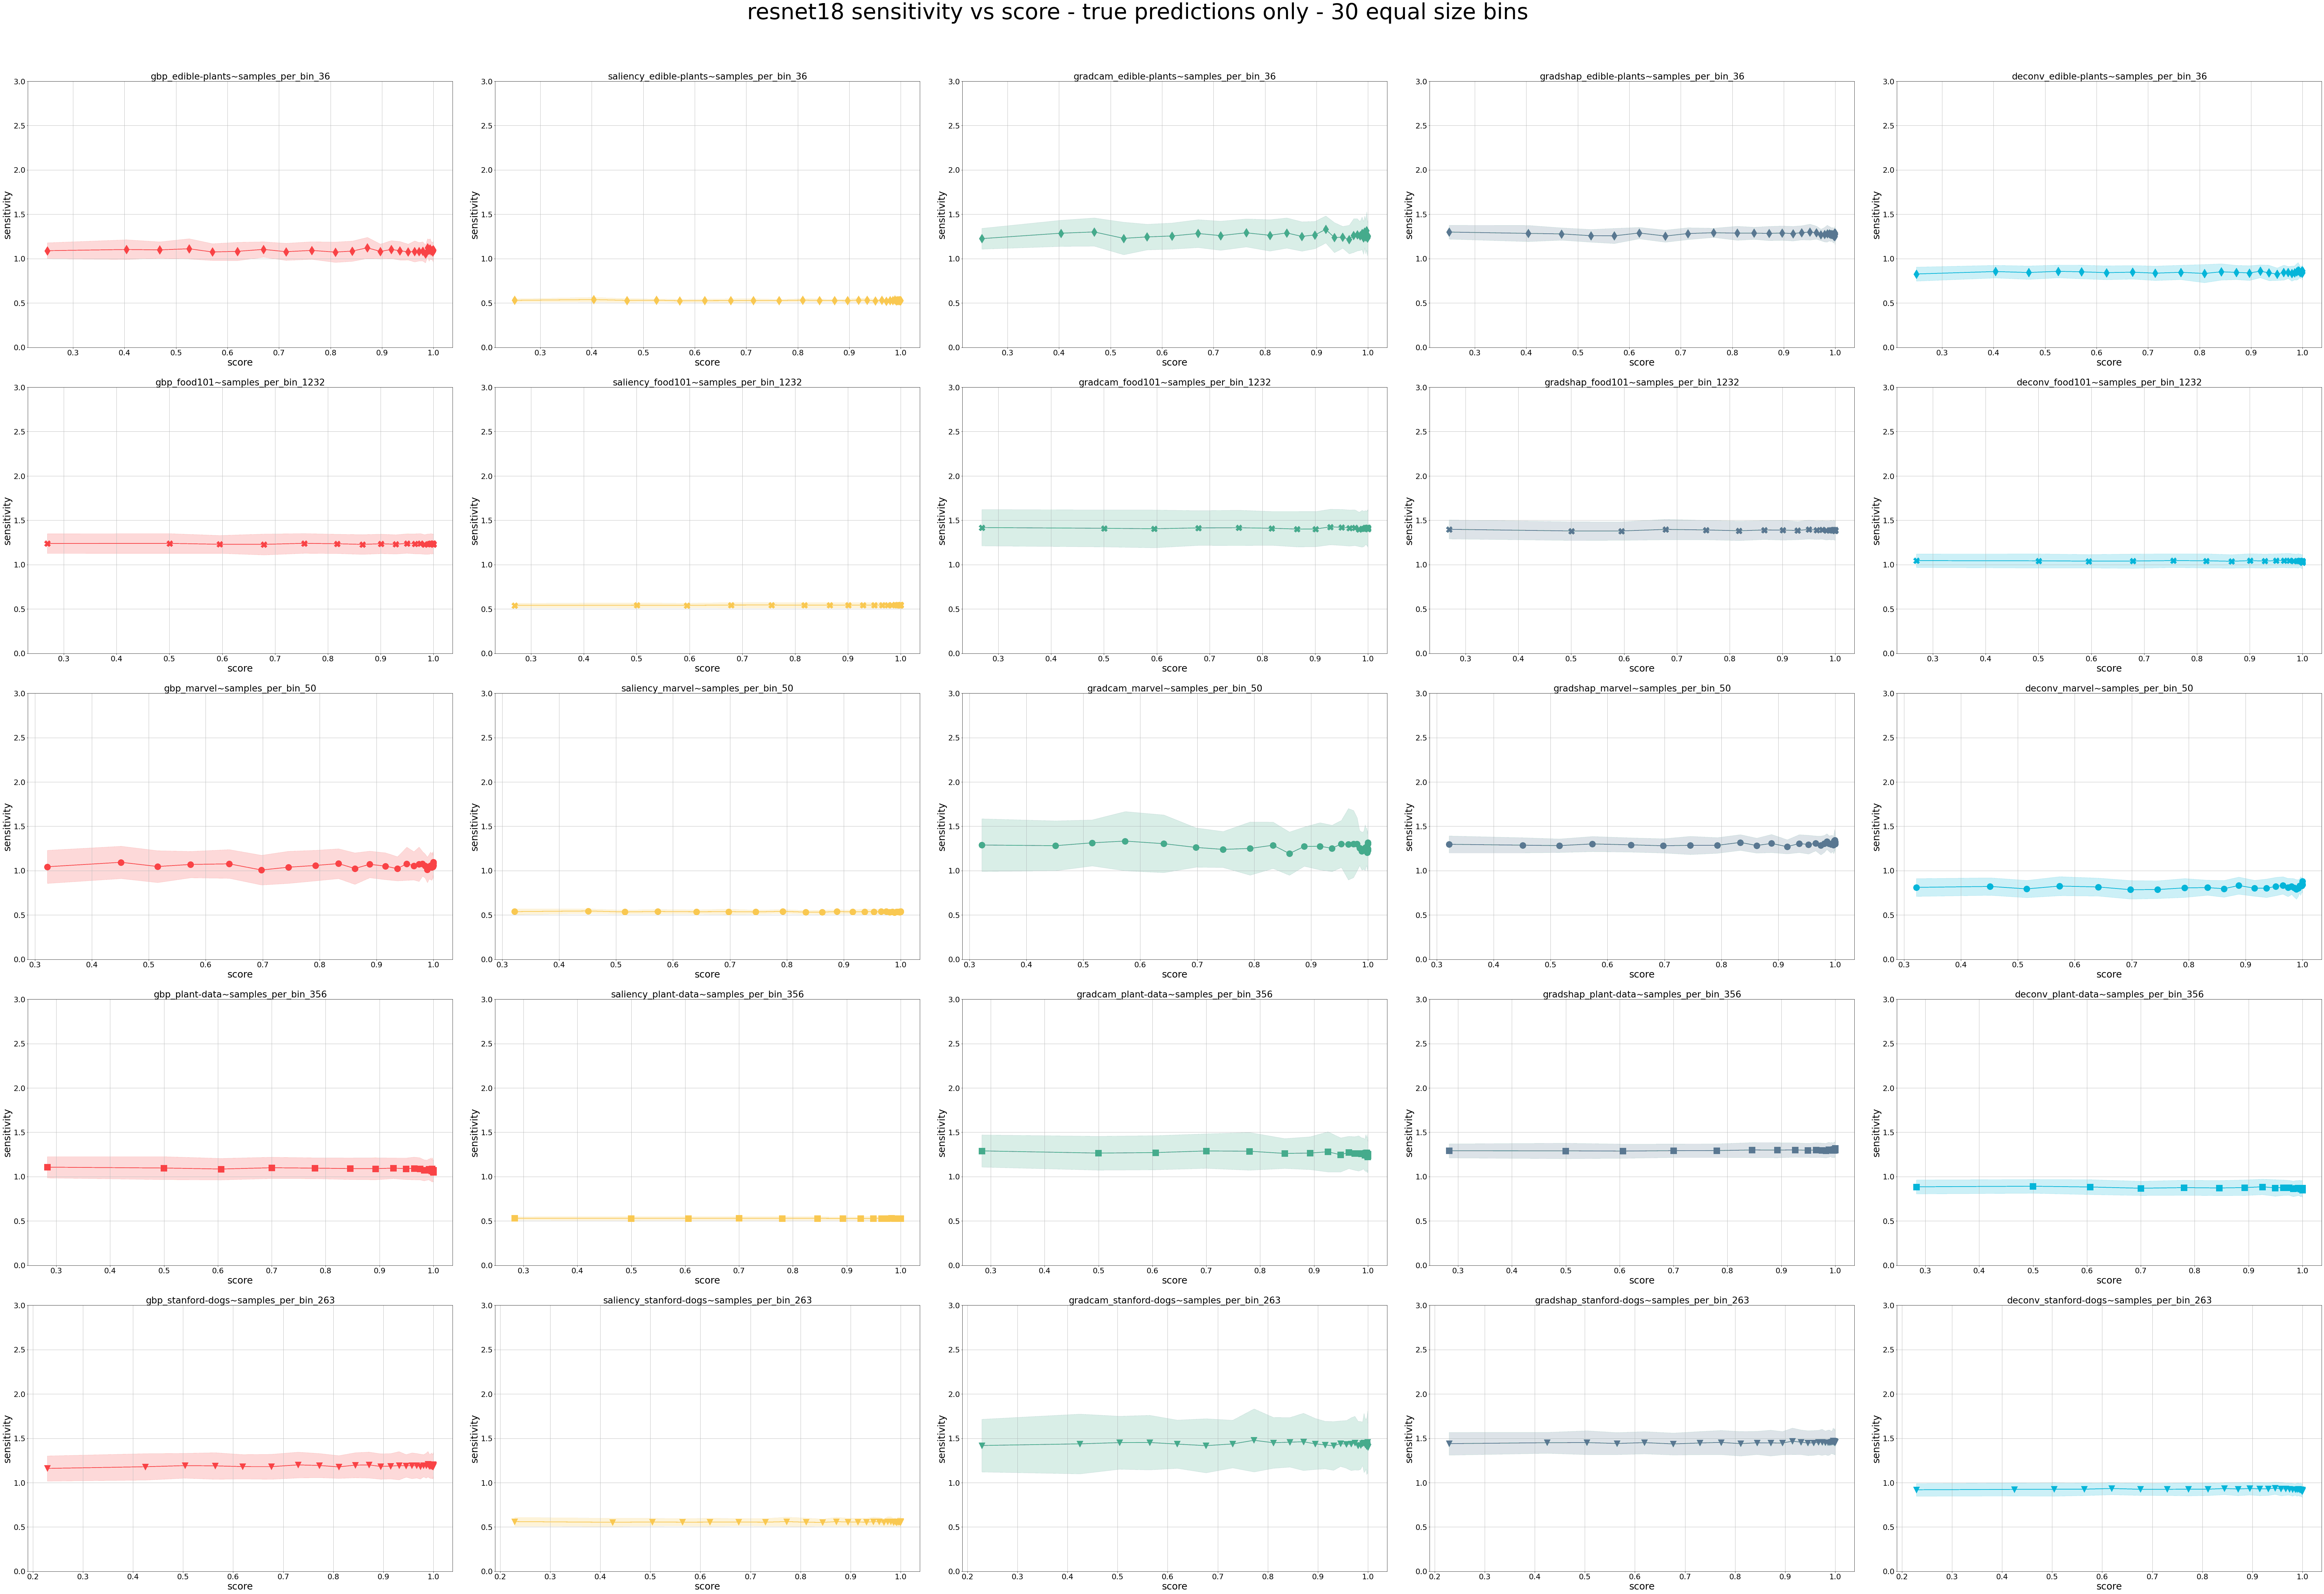
\includegraphics[width=\textwidth]{results/metrics/resnet18-sensitivity vs score - true predictions only - 30 equal size bins.png}
    \caption{Sensitivity scores (with standard deviation) on \textit{ResNet18} architecture. All scores are the mean value for the particular model and are related to that models' predicted scores (x-axis). Each data point is a mean value of the same amount of samples per dataset. Amounts differ between datasets to always split the results into 30 equally-sized bins.}\label{fig:resnet-sens-std}
\end{figure}

\begin{figure}[ht]
  \centering
    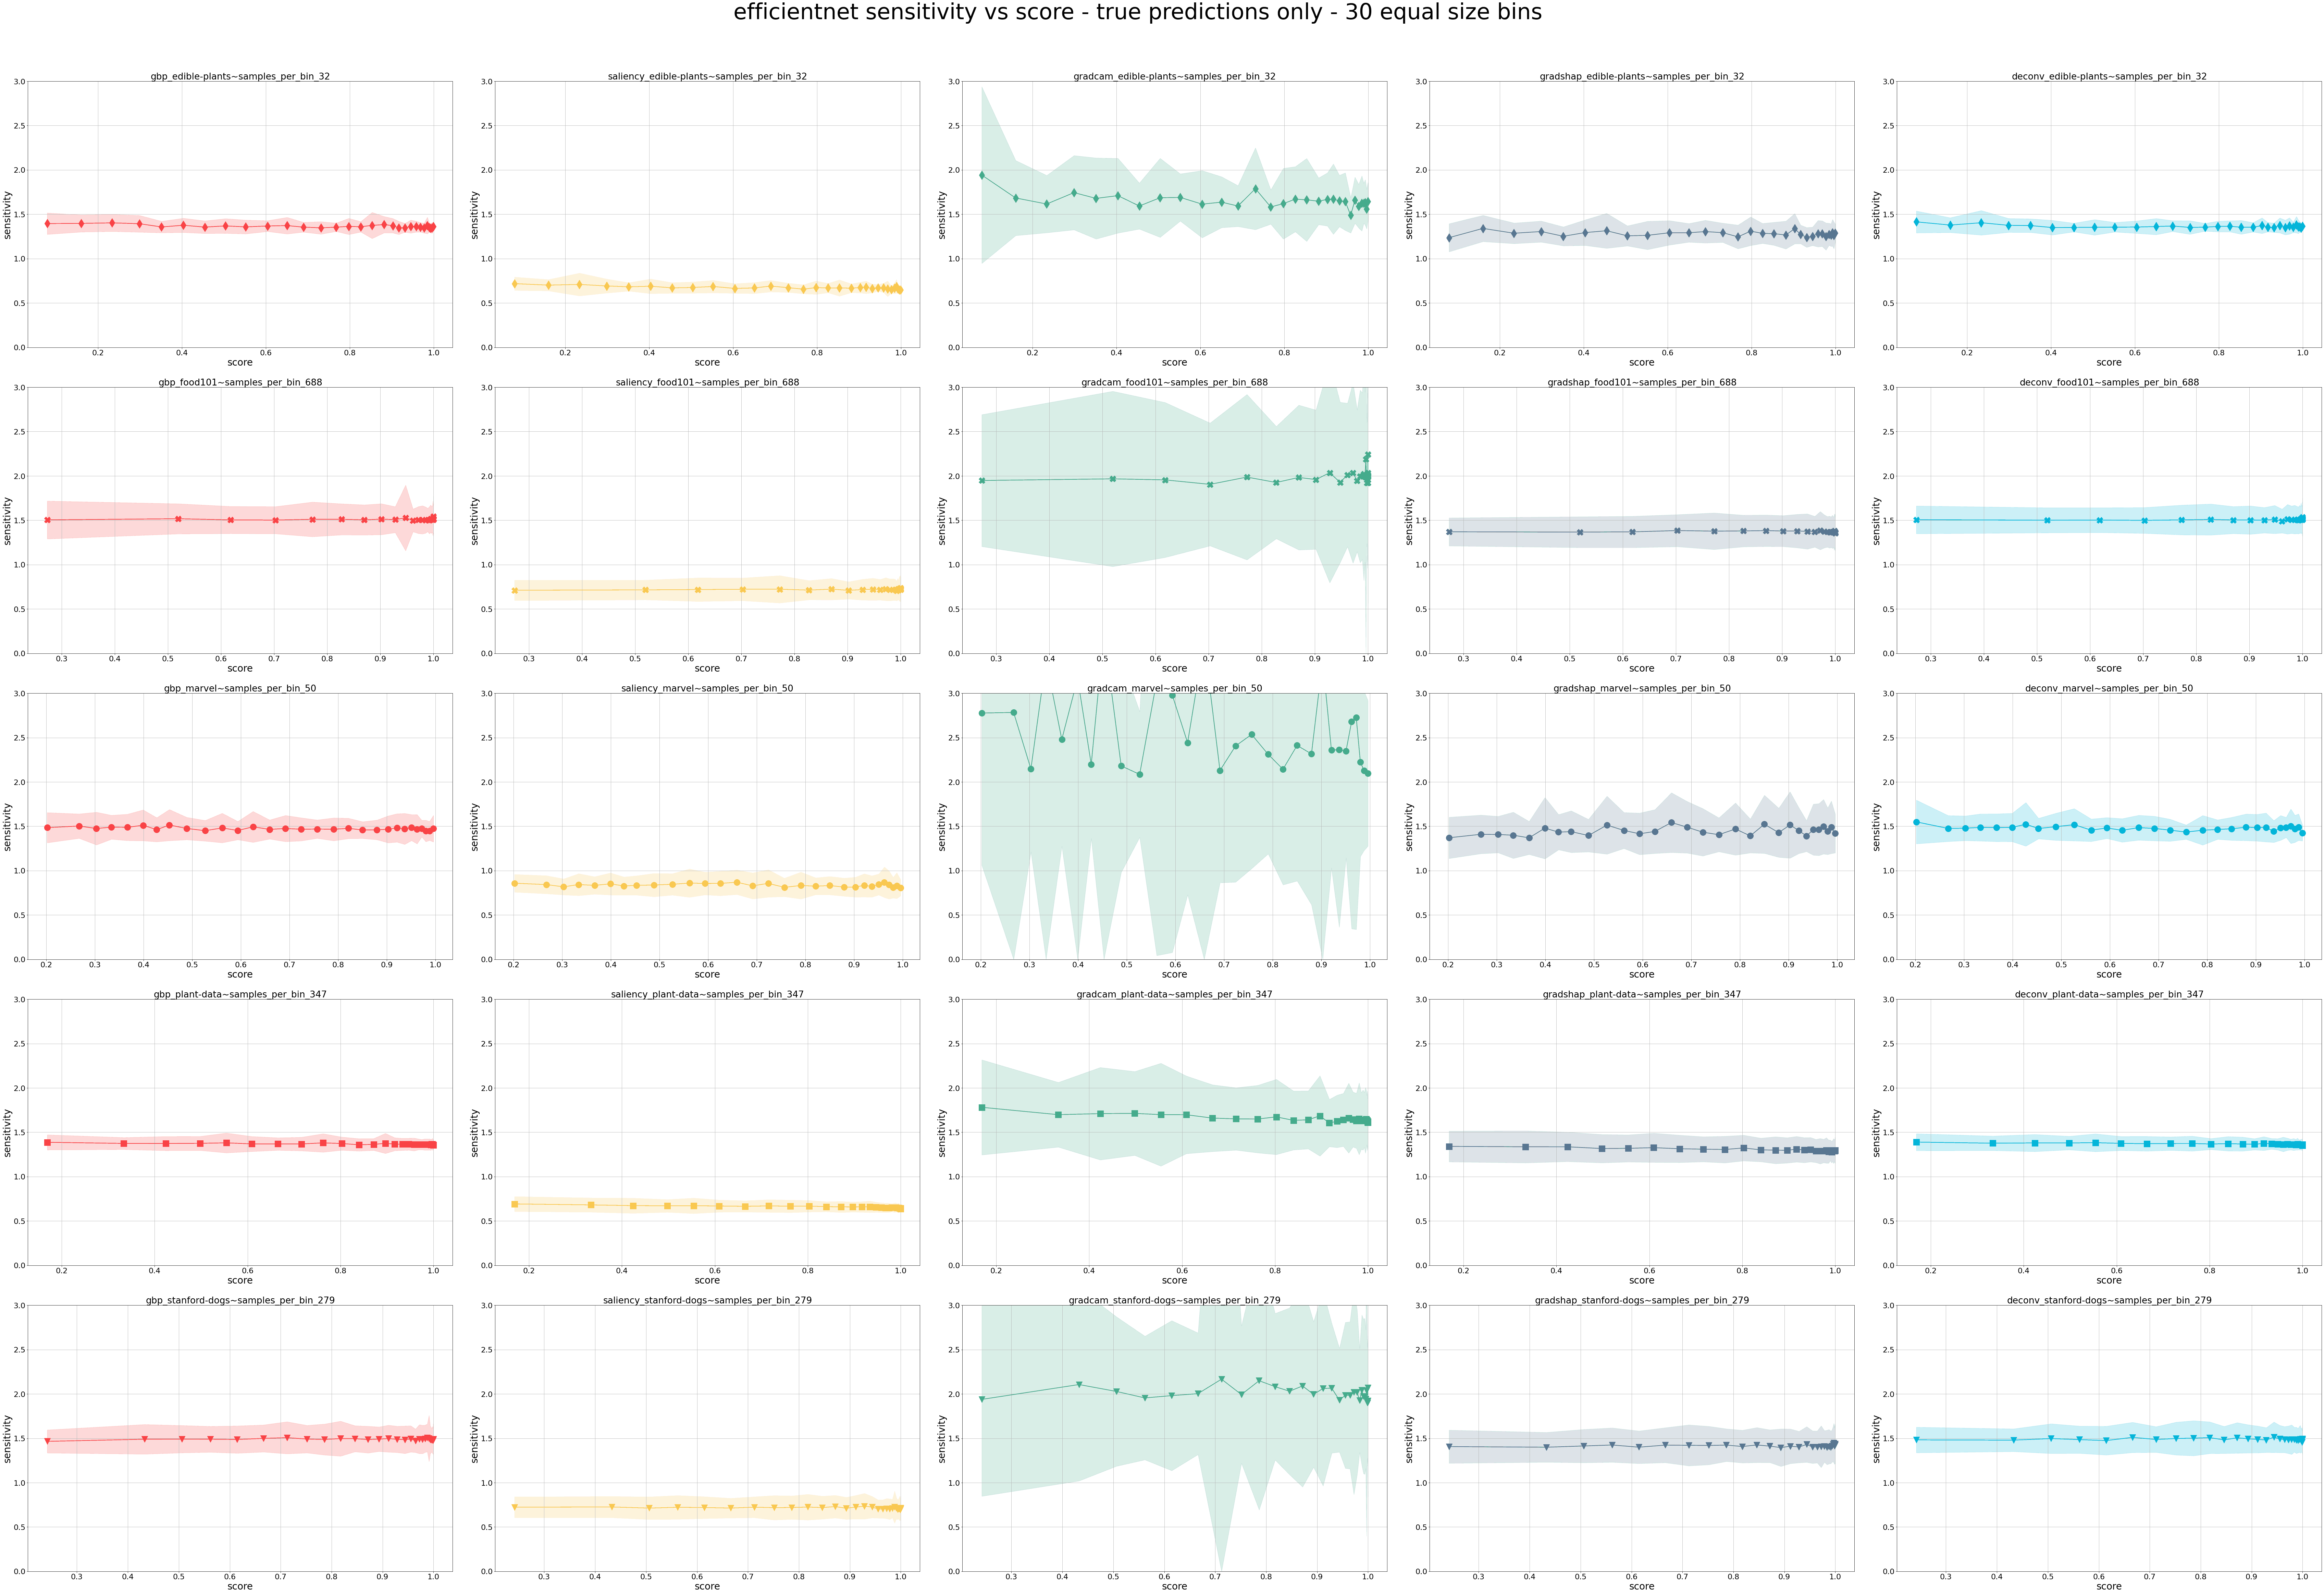
\includegraphics[width=\textwidth]{results/metrics/efficientnet-sensitivity vs score - true predictions only - 30 equal size bins.png}
    \caption{Sensitivity scores (with standard deviation) on \textit{EfficientNet B0} architecture. All scores are the mean value for the particular model and are related to that models' predicted scores (x-axis). Each data point is a mean value of the same amount of samples per dataset. Amounts differ between datasets to always split the results into 30 equally-sized bins.}\label{fig:efficientnet-sens-std}
\end{figure}